\documentclass{pengaturan/skripsi}

\usepackage{longtable}
\usepackage{array}
\usepackage{xcolor}
\usepackage{tikz}
\usetikzlibrary{shapes.geometric,arrows.meta,positioning,fit,calc,backgrounds}

%===========================================================
% Definisi Data Peneliti, Judul, Pembimbing dan Penguji
%-----------------------------------------------------------
\titleskripsi{ANALISIS QOS JARINGAN BERBASIS CROWDSOURCING PADA APLIKASI PRESENSI MENGGUNAKAN K-MEANS}

\fullname{ABD. ROUF}
\idnum{223140118}

\yearsubmit{2026}
\program{Informatika}
\dept{Informatika}
\faculty{Fakultas Teknik dan Informatika}
\university{Institut Teknologi dan Bisnis Widya Gama}
\city{Lumajang}

\firstsupervisor{Nama Dosen Pembimbing, S.Kom., M.Kom.}
\secondsupervisor{-}
\firstexaminer{Nama Dosen Penguji 1, S.Kom., M.Kom.}
\secondexaminer{Nama Dosen Penguji 2, S.Kom., M.Kom.}
%-----------------------------------------------------------
% End Definisi Data Peneliti, Judul, Pembimbing dan Penguji
%===========================================================

\hypersetup{
    pdftitle={Analisis QoS Jaringan Berbasis Crowdsourcing pada Aplikasi Presensi Menggunakan K-Means},
    pdfauthor={Abd. Rouf},
    pdfsubject={Proposal Skripsi}
}

\begin{document}
    % Sampul proposal untuk ujian proposal skripsi (Pedoman 4.3 no. 1)
    \coverproposal

    % Halaman Pengesahan Proposal, Pengesahan Ujian Proposal, dan Persetujuan
    % Pembimbing diunduh dari https://siakadv2.itbwigalumajang.ac.id lalu
    % disisipkan saat mencetak (Pedoman 2.2 dan 4.3).
    \chapter*{KATA PENGANTAR}
\phantomsection
\addcontentsline{toc}{chapter}{KATA PENGANTAR}

% Pedoman 4.3 no. 5: maksimal 2 halaman; terima kasih cukup kepada 5 pihak berikut.
% Ganti teks dalam {[...]} dengan nama lengkap dan gelar. Kurung kurawal wajib selama
% teks masih diawali "[", karena "\item [..." dibaca LaTeX sebagai label nomor.
Puji syukur penulis panjatkan kepada Tuhan Yang Maha Esa karena atas rahmat-Nya penulis dapat menyelesaikan proposal skripsi yang berjudul ``Analisis QoS Jaringan Berbasis \textit{Crowdsourcing} pada Aplikasi Presensi Menggunakan K-Means''. Proposal ini disusun sebagai salah satu syarat untuk mengikuti ujian proposal skripsi pada Program Studi Informatika, Fakultas Teknik dan Informatika, Institut Teknologi dan Bisnis Widya Gama Lumajang.

Penulis mengucapkan terima kasih kepada:
\begin{enumerate}[topsep=0pt,itemsep=0pt]
    \item {[Nama Rektor]}, selaku Rektor Institut Teknologi dan Bisnis Widya Gama Lumajang.
    \item {[Nama Dekan]}, selaku Dekan Fakultas Teknik dan Informatika.
    \item {[Nama Ketua Program Studi]}, selaku Ketua Program Studi Informatika.
    \item {[Nama Dosen Pembimbing]}, selaku Dosen Pembimbing.
    \item Orang tua dan keluarga penulis.
\end{enumerate}

Penulis menyadari bahwa proposal ini masih memiliki kekurangan. Oleh karena itu, kritik dan saran yang membangun sangat penulis harapkan.

\vspace{1cm}
\begin{flushright}
Lumajang, [tanggal] 2026\\[2cm]
Penulis
\end{flushright}

    \pagebreak

    %===========================================================
    % Daftar isi, daftar tabel, daftar gambar
    % Setiap baris bisa diklik (linktoc=all di pengaturan/skripsi.cls)
    %-----------------------------------------------------------
    \tocchapter{DAFTAR ISI}
    \tableofcontents
    \pagebreak

    \tocchapter{DAFTAR TABEL}
    \listoftables
    \pagebreak

    \tocchapter{DAFTAR GAMBAR}
    \listoffigures
    \pagebreak

    \pagenumbering{arabic}
    %-----------------------------------------------------------
    % End Daftar isi, daftar tabel, daftar gambar
    %===========================================================

    %===========================================================
    % Bab 1-3 (Pedoman 4.1: Bab 1 maks. 5 hlm, Bab 2 dan 3 maks. 15 hlm)
    %-----------------------------------------------------------
    \chapter{PENDAHULUAN}

\section{Latar Belakang Masalah}
Aplikasi presensi berbasis \textit{mobile} kini banyak digunakan perusahaan untuk mencatat kehadiran karyawan yang bekerja di lebih dari satu lokasi. Aplikasi semacam ini mengirim data presensi, foto, dan lokasi ke server melalui jaringan Wi-Fi atau seluler, sehingga keberhasilannya bergantung pada kualitas jaringan di tempat karyawan berada \parencite{ismail2023presensi,rokhman2026personalia}. Ketika koneksi di lapangan tidak stabil, data presensi dapat gagal atau terlambat sampai ke server, sehingga beberapa penelitian menambahkan mode \textit{offline} yang menyimpan data di perangkat terlebih dahulu lalu mengirimkannya ketika koneksi kembali tersedia \parencite{indah2025offline,rokhman2026personalia}.

PT Semeru Agung Mandiri menghadapi kondisi yang sama. Karyawannya melakukan presensi melalui aplikasi Android dari kantor, posko, dan gudang yang kondisi jaringannya berbeda-beda. Aplikasi presensi perusahaan, yang dibangun oleh penulis dengan Flutter dan server PocketBase, sengaja dirancang dengan arsitektur \textit{offline-first} karena sebelumnya muncul keluhan presensi gagal terkirim di lokasi tertentu. Data presensi kini disimpan terlebih dahulu di perangkat lalu dikirim melalui antrean sinkronisasi ketika jaringan tersedia. Arsitektur ini berhasil mencegah presensi hilang, tetapi hanya mengatasi gejalanya. Penyebabnya, yaitu kualitas jaringan yang buruk, tetap ada dan tidak pernah diukur. Permasalahan yang muncul dari kondisi tersebut dirangkum pada Tabel~\ref{tab:permasalahan}.

\begin{table}[!ht]
\centering
\caption{Permasalahan dan Dampaknya bagi Perusahaan}
\label{tab:permasalahan}
\begin{tabular}{>{\centering\arraybackslash}p{0.8cm}>{\raggedright\arraybackslash}p{5.0cm}>{\raggedright\arraybackslash}p{7.14cm}}
\toprule
\textbf{No.} & \textbf{Permasalahan} & \textbf{Dampak} \\ \midrule
1. & Presensi di lokasi tertentu gagal atau terlambat terkirim & Rekap kehadiran untuk penggajian terlambat atau tidak lengkap; HRD memeriksa manual \\ \garis
2. & Tidak ada data kualitas jaringan per lokasi dan jam & Lokasi yang perlu perbaikan tidak diketahui; biaya Wi-Fi atau \textit{repeater} bisa salah sasaran \\ \garis
3. & Keluhan presensi tidak bisa dibuktikan dengan data & Sulit membedakan keterlambatan karena jaringan dari sebab lain \\ \garis
4. & Pengukuran manual ke setiap lokasi mahal dan lama & Pengukuran sesaat di satu titik tidak mewakili seluruh lokasi dan jam kerja \\ \bottomrule
\end{tabular}
\par\vspace{3pt}
{\raggedright\footnotesize Sumber: pengamatan penulis sebagai pengembang aplikasi presensi, 2026\par}
\end{table}

Berdasarkan Tabel~\ref{tab:permasalahan} dapat dinyatakan bahwa inti permasalahannya adalah \textbf{perusahaan belum memiliki data objektif tentang kualitas jaringan di setiap lokasi kerja}, yaitu lokasi mana yang jaringannya buruk, pada jam berapa, melalui jenis jaringan apa, dan seberapa buruk.

Kualitas jaringan sebenarnya dapat diukur secara objektif dengan parameter \textit{Quality of Service} (QoS), yaitu \textit{delay}, \textit{jitter}, \textit{packet loss}, dan \textit{throughput}, yang hasilnya dikategorikan menurut standar TIPHON \parencite{etsi1999tiphon,rosid2023qos}. Namun, penelitian QoS di Indonesia umumnya mengukur satu jaringan di satu lokasi dengan menangkap lalu lintas menggunakan Wireshark \parencite{rosid2023qos,fiqria2024qos,basmar2026jamsibuk} atau dengan aplikasi pengukur seperti speedtest dan nPerf \parencite{ramayanti2024qos,ainina2024qos4g}. Cara ini dilakukan manual di titik dan waktu tertentu, sehingga tidak cocok untuk perusahaan dengan banyak lokasi, padahal kualitas jaringan berubah menurut waktu. \textcite{basmar2026jamsibuk} menemukan bahwa pada jam sibuk \textit{packet loss} mencapai 26,5\% dan \textit{delay} 485 ms, keduanya kategori buruk menurut TIPHON. Aplikasi pengukur kecepatan juga mengukur ke servernya sendiri, bukan ke server perusahaan yang dipakai untuk presensi.

Kendala tersebut dapat diatasi dengan pengukuran jaringan berbasis \textit{crowdsourcing}, yaitu pengukuran yang dijalankan langsung di perangkat banyak pengguna sehingga mencerminkan kondisi nyata yang mereka alami \parencite{wamser2021crowd}. Pengukuran dapat berjalan otomatis dari lalu lintas aplikasi tanpa tindakan pengguna, seperti dibuktikan \textcite{wu2017mopeye} melalui lebih dari lima juta pengukuran dari 2.351 ponsel. Data sebanyak itu perlu dikelompokkan agar mudah ditindaklanjuti. Algoritma K-Means telah digunakan untuk mengelompokkan kualitas internet seluler 17 kabupaten/kota menjadi tiga klaster \parencite{irwansyah2025kmeans} dan pemakaian \textit{bandwidth} 32 organisasi perangkat daerah menjadi kategori tinggi, sedang, dan rendah \parencite{mubarak2023kmeans}.

Meskipun demikian, terdapat celah yang belum diisi oleh penelitian-penelitian tersebut. Pertama, penelitian QoS yang ada mengukur secara manual di satu titik pada waktu tertentu \parencite{fiqria2024qos,rosid2023qos}. Kedua, penelitian K-Means kualitas jaringan memakai data pihak ketiga (Ookla Open Data) atau data perangkat pemantau jaringan, bukan data dari aplikasi yang dipakai sehari-hari \parencite{irwansyah2025kmeans,mubarak2023kmeans}. Ketiga, penelitian aplikasi presensi hanya menangani koneksi buruk dengan mode \textit{offline} tanpa mengukur jaringannya \parencite{indah2025offline,rokhman2026personalia}. Sepanjang penelusuran penulis, belum ditemukan penelitian yang memanfaatkan aplikasi presensi perusahaan sebagai alat ukur QoS berbasis \textit{crowdsourcing} lalu mengelompokkan hasilnya dengan K-Means.

Penelitian ini perlu dilakukan karena tiga alasan. Pertama, presensi merupakan dasar rekap kehadiran dan penggajian, sehingga lokasi dengan jaringan buruk berdampak langsung pada administrasi perusahaan dan karyawan. Kedua, perbaikan jaringan memerlukan biaya, sehingga harus diarahkan ke lokasi dan jam yang terbukti bermasalah, bukan berdasarkan perkiraan. Ketiga, aplikasi presensi sudah dipakai setiap hari di semua lokasi kerja, sehingga dapat menjadi alat ukur yang murah tanpa mengirim petugas ke setiap lokasi. Tanpa penelitian ini, perusahaan hanya mengetahui masalah jaringan dari keluhan, setelah presensi telanjur gagal terkirim.

Oleh karena itu, penelitian ini mengembangkan modul telemetri pada aplikasi presensi PT Semeru Agung Mandiri. Modul tersebut mencatat \textit{delay}, \textit{jitter}, tingkat kegagalan, \textit{throughput}, dan lama putus koneksi secara otomatis dan anonim tanpa mengubah alur presensi. Data yang terkumpul selama empat minggu dikategorikan menurut standar TIPHON, lalu dikelompokkan dengan K-Means per lokasi kerja, jenis jaringan, dan waktu. Hasil yang dituju adalah peta kualitas jaringan perusahaan, yaitu daftar lokasi dan jam berkualitas baik, sedang, dan buruk sebagai dasar perbaikan jaringan.

\section{Batasan Masalah}
Agar penelitian ini fokus dan terarah, ruang lingkupnya dibatasi sebagai berikut:
\begin{enumerate}
    \item Penelitian dilakukan pada aplikasi presensi Android PT Semeru Agung Mandiri (Flutter, Isar, dan PocketBase). Perangkat iOS tidak diteliti.
    \item Kualitas jaringan yang diukur adalah jalur komunikasi dari perangkat karyawan ke server perusahaan melalui HTTPS, bukan akses internet secara umum.
    \item Parameter yang diukur adalah \textit{delay} (\textit{round-trip time} tingkat aplikasi), \textit{jitter}, tingkat kegagalan pengiriman sebagai pengganti \textit{packet loss}, \textit{throughput} unggah, dan lama putus koneksi.
    \item Data dikumpulkan selama empat minggu hari kerja dan hanya ketika aplikasi sedang berjalan. Sinkronisasi latar belakang (WorkManager) tidak dicatat.
    \item Data bersifat anonim tanpa nama, email, koordinat GPS, maupun foto. Lokasi diwakili kode lokasi kerja.
    \item Kategori kualitas mengacu pada standar TIPHON, dan pengelompokan memakai K-Means dengan jumlah klaster dari metode \textit{elbow} dan nilai \textit{silhouette}. Penelitian tidak melakukan perbaikan jaringan, tetapi memberikan rekomendasi bagi perusahaan.
\end{enumerate}

\section{Rumusan Masalah}
Rumusan masalah dalam penelitian ini adalah sebagai berikut:
\begin{enumerate}
    \item Bagaimana mengembangkan modul telemetri QoS pada aplikasi presensi yang hasil pengukurannya valid dan tidak mengganggu alur presensi karyawan?
    \item Bagaimana kualitas jaringan di setiap lokasi kerja PT Semeru Agung Mandiri berdasarkan nilai \textit{delay}, \textit{jitter}, tingkat kegagalan, dan \textit{throughput} menurut kategori TIPHON?
    \item Bagaimana hasil pengelompokan kualitas jaringan per lokasi kerja, jenis jaringan, dan waktu menggunakan K-Means, serta sejauh mana kesesuaiannya dengan kategori TIPHON dan keterangan HRD?
\end{enumerate}

\section{Tujuan Penelitian}
Secara umum, penelitian ini bertujuan menyediakan data objektif tentang kualitas jaringan di setiap lokasi kerja dengan aplikasi presensi sebagai alat ukur. Sejalan dengan rumusan masalah, tujuan khususnya adalah:
\begin{enumerate}
    \item Mengembangkan dan memvalidasi modul telemetri QoS pada aplikasi presensi sebagai alat ukur yang akurat dan aman.
    \item Mengukur \textit{delay}, \textit{jitter}, tingkat kegagalan, dan \textit{throughput} jaringan di setiap lokasi kerja, lalu mengategorikannya menurut standar TIPHON, sehingga diketahui lokasi dengan kualitas jaringan buruk.
    \item Mengelompokkan kualitas jaringan per lokasi kerja, jenis jaringan, dan waktu menggunakan K-Means, lalu membandingkan hasilnya dengan kategori TIPHON dan keterangan HRD, sehingga diketahui pola lokasi dan jam yang bermasalah.
\end{enumerate}

\section{Manfaat Penelitian}
Manfaat penelitian ini terdiri atas manfaat teoritis dan praktis sebagai berikut:
\begin{enumerate}
    \item \textbf{Manfaat Teoritis}\\
    Penelitian ini memberikan cara pengukuran QoS berbasis \textit{crowdsourcing} yang memakai aplikasi operasional sebagai alat ukur, sebagai alternatif pengukuran manual di satu titik, dan penerapan K-Means pada data QoS dari perangkat pengguna.
    \item \textbf{Manfaat Praktis}
    \begin{enumerate}[label=\alph*.]
        \item Bagi perusahaan, peta kualitas jaringan menjadi dasar perbaikan jaringan.
        \item Bagi HRD, data per lokasi dan jam membantu menelusuri keluhan presensi gagal terkirim.
        \item Bagi pengembang, modul telemetri dapat terus memantau jaringan.
    \end{enumerate}
\end{enumerate}

    \chapter{TINJAUAN PUSTAKA}

\section{Landasan Teori}
Landasan teori berikut membahas konsep yang digunakan dalam penelitian, mulai dari objek penelitian (aplikasi presensi \textit{mobile} dan arsitektur \textit{offline-first}), apa yang diukur (QoS dan standar TIPHON), cara mengukur (pengukuran berbasis \textit{crowdsourcing} dan telemetri pasif), cara menganalisis (K-Means, metode \textit{elbow}, dan nilai \textit{silhouette}), hingga metode penelitian dan aspek pelindungan data pribadi.

\subsection{Aplikasi Presensi Mobile dan Arsitektur Offline-First}
Aplikasi presensi \textit{mobile} adalah aplikasi pada telepon pintar yang digunakan karyawan untuk mencatat kehadiran, biasanya dilengkapi validasi lokasi dengan GPS dan foto. \textcite{ismail2023presensi} membangun aplikasi presensi berbasis Flutter dan \textit{library} Geolocator untuk menggantikan mesin sidik jari yang datanya harus direkap secara manual, sedangkan \textcite{rokhman2026personalia} membangun sistem personalia multiplatform dengan presensi berbasis \textit{geofence}, verifikasi wajah, dan pelacakan lokasi tenaga penjual. Kedua aplikasi tersebut bergantung pada jaringan untuk mengirim data ke server.

Masalah koneksi di lapangan diatasi dengan mode \textit{offline}. \textcite{indah2025offline} mengembangkan aplikasi absensi berbasis QR Code yang menyimpan data secara lokal ketika koneksi tidak tersedia dan menyinkronkannya ke server ketika koneksi kembali, karena perusahaan memiliki banyak lokasi kerja dengan koneksi yang tidak stabil. \textcite{rokhman2026personalia} menerapkan penyimpanan lokal SQLite dan penanda \texttt{client\_event\_id} agar sinkronisasi tetap konsisten ketika koneksi tidak stabil. Pendekatan yang menjadikan penyimpanan lokal sebagai sumber data utama dan sinkronisasi sebagai proses susulan disebut \textit{offline-first} \parencite{devina2026offlinefirst}.

Aplikasi presensi PT Semeru Agung Mandiri menerapkan arsitektur \textit{offline-first}. Setiap presensi disimpan terlebih dahulu di basis data lokal Isar, dimasukkan ke antrean sinkronisasi, lalu dikirim ke server PocketBase melalui HTTPS ketika perangkat terhubung ke jaringan. Antrean ini mencatat setiap percobaan pengiriman beserta hasilnya. Dalam penelitian ini, percobaan pengiriman tersebut dimanfaatkan sebagai sumber data kualitas jaringan tanpa mengubah cara kerja antrean.

Aplikasi juga memvalidasi lokasi dengan \textit{geofence}, yaitu presensi hanya dapat dilakukan jika perangkat berada di dalam radius lokasi kerja yang dipilih. Terdapat tiga pengecualian: (1) mode tugas luar kota atau lapangan (GAMAS), yang membolehkan presensi dari mana saja dengan menuliskan lokasi dan keterangan tugas untuk disetujui admin; (2) karyawan yang diberi izin lokasi fleksibel oleh admin, yang tidak diperiksa radiusnya sama sekali; dan (3) titik sementara yang dibuat admin dengan radius dan batas waktu sendiri. Presensi tidak mewajibkan Wi-Fi kantor. Selama berada di dalam radius, karyawan boleh memakai Wi-Fi maupun data seluler, dan aplikasi hanya mencatat apakah Wi-Fi yang terhubung adalah Wi-Fi kantor berdasarkan BSSID. Pemeriksaan \textit{geofence} tetap berjalan ketika perangkat tidak terhubung ke internet, karena posisi dibaca dari satelit GPS dan daftar lokasi kerja tersimpan di basis data lokal, sehingga presensi \textit{offline} di lokasi kerja tetap tervalidasi. Aturan-aturan ini menentukan apakah lokasi sebuah sampel pengukuran dapat dipercaya, sehingga diperhitungkan dalam rancangan data dan analisis pada Bab 3.

\subsection{Quality of Service}
\label{subsec:qos}
\textit{Quality of Service} (QoS) adalah cara mengukur seberapa baik jaringan menyediakan layanan pengiriman data, yang dinyatakan dengan sejumlah parameter yang dapat diukur \parencite{rosid2023qos}. Parameter QoS yang umum digunakan adalah sebagai berikut \parencite{etsi1999tiphon,rosid2023qos,basmar2026jamsibuk}.
\begin{enumerate}
    \item \textbf{\textit{Delay}}, yaitu waktu yang dibutuhkan data untuk menempuh jarak dari asal ke tujuan. Pada pengukuran pulang-pergi, \textit{delay} dinyatakan sebagai \textit{round-trip time} (RTT), yaitu selisih waktu antara permintaan dikirim dan balasan diterima:
    \begin{equation}
    d = t_{\mathrm{terima}} - t_{\mathrm{kirim}}
    \label{eq:delay}
    \end{equation}
    dengan $d$ adalah \textit{delay} dalam milidetik (ms), $t_{\mathrm{kirim}}$ adalah waktu permintaan dikirim, dan $t_{\mathrm{terima}}$ adalah waktu balasan diterima.
    \item \textbf{\textit{Jitter}}, yaitu variasi \textit{delay} antarpaket atau antarpengukuran yang berurutan. Semakin besar \textit{jitter}, semakin tidak stabil jaringan:
    \begin{equation}
    J = \frac{1}{n-1}\sum_{i=2}^{n} \left| d_i - d_{i-1} \right|
    \label{eq:jitter}
    \end{equation}
    dengan $J$ adalah \textit{jitter} (ms), $d_i$ adalah \textit{delay} pengukuran ke-$i$, dan $n$ adalah jumlah pengukuran.
    \item \textbf{\textit{Packet loss}}, yaitu persentase paket yang hilang dan tidak sampai ke tujuan:
    \begin{equation}
    PL = \frac{\text{paket dikirim} - \text{paket diterima}}{\text{paket dikirim}} \times 100\%
    \label{eq:packetloss}
    \end{equation}
    \item \textbf{\textit{Throughput}}, yaitu kecepatan nyata pengiriman data, dihitung dari jumlah data yang berhasil dikirim dibagi waktu pengiriman:
    \begin{equation}
    T = \frac{B \times 8}{\Delta t}
    \label{eq:throughput}
    \end{equation}
    dengan $T$ adalah \textit{throughput} dalam kbps, $B$ adalah jumlah data terkirim dalam \textit{byte}, dan $\Delta t$ adalah lama pengiriman dalam milidetik.
\end{enumerate}

\textit{Packet loss} pada Persamaan~(\ref{eq:packetloss}) dihitung per paket di tingkat jaringan. Aplikasi Android biasa tidak dapat melihat paket tanpa akses khusus, sehingga dalam penelitian ini \textit{packet loss} diganti dengan tingkat kegagalan pengiriman di tingkat aplikasi, yaitu persentase permintaan yang gagal karena masalah jaringan. Keduanya sama-sama menggambarkan data yang tidak sampai, tetapi tingkat kegagalan lebih kasar karena satu permintaan terdiri atas banyak paket. Penggantian ini dinyatakan sebagai keterbatasan penelitian.

\subsection{Standar TIPHON}
\textit{Telecommunications and Internet Protocol Harmonization Over Networks} (TIPHON) adalah dokumen ETSI yang membahas aspek umum QoS pada jaringan berbasis IP \parencite{etsi1999tiphon}. Penelitian QoS di Indonesia menggunakan kategori TIPHON untuk menilai \textit{delay}, \textit{jitter}, \textit{packet loss}, dan \textit{throughput} ke dalam indeks 1 sampai 4 \parencite{rosid2023qos,fiqria2024qos,ramayanti2024qos,basmar2026jamsibuk}. Kategori yang digunakan dalam penelitian ini ditunjukkan pada Tabel~\ref{tab:tiphon}.

\begin{table}[!ht]
\centering
\caption{Kategori Parameter QoS Menurut Standar TIPHON}
\label{tab:tiphon}
\begin{tabular}{>{\raggedright\arraybackslash}p{2.1cm}>{\centering\arraybackslash}p{1.85cm}>{\centering\arraybackslash}p{1.85cm}>{\centering\arraybackslash}p{1.9cm}>{\centering\arraybackslash}p{2.98cm}>{\centering\arraybackslash}p{1.2cm}}
\toprule
\textbf{Kategori} & \textbf{\textit{Delay}} & \textbf{\textit{Jitter}} & \textbf{\textit{Packet Loss}} & \textbf{\textit{Throughput}} & \textbf{Indeks} \\ \midrule
Sangat bagus & $<$ 150 ms & 0 ms & 0\% & $>$ 2,1 Mbps & 4 \\ \garis
Bagus & 150--300 ms & 0--75 ms & 3\% & 1,2--2,1 Mbps & 3 \\ \garis
Sedang & 300--450 ms & 75--125 ms & 15\% & 700 kbps--1,2 Mbps & 2 \\ \garis
Jelek & $>$ 450 ms & 125--225 ms & 25\% & $<$ 700 kbps & 1 \\ \bottomrule
\end{tabular}
\par\vspace{3pt}
{\raggedright\footnotesize Sumber: \textcite{etsi1999tiphon} dalam \textcite{rosid2023qos}\par}
\end{table}

Berdasarkan Tabel~\ref{tab:tiphon} dapat dinyatakan bahwa setiap parameter memiliki satuan dan ambang yang berbeda, tetapi semuanya dikonversi ke indeks yang sama, yaitu 1 sampai 4. Nilai \textit{packet loss} pada tabel merupakan batas bawah setiap kategori, sehingga dalam penelitian ini kategori sangat bagus diartikan kurang dari 3\%, bagus 3\% sampai kurang dari 15\%, sedang 15\% sampai kurang dari 25\%, dan jelek 25\% atau lebih. Indeks keseluruhan diperoleh dari rata-rata indeks keempat parameter, lalu ditafsirkan dengan kategori pada Tabel~\ref{tab:tiphon_total}.

\begin{table}[!ht]
\centering
\caption{Kategori Indeks Keseluruhan TIPHON}
\label{tab:tiphon_total}
\begin{tabular}{>{\centering\arraybackslash}p{4.0cm}>{\centering\arraybackslash}p{4.0cm}>{\raggedright\arraybackslash}p{4.94cm}}
\toprule
\textbf{Rata-rata Indeks} & \textbf{Persentase} & \textbf{Kategori} \\ \midrule
3,80--4,00 & 95--100\% & Sangat memuaskan \\ \garis
3,00--3,79 & 75--94,75\% & Memuaskan \\ \garis
2,00--2,99 & 50--74,75\% & Kurang memuaskan \\ \garis
1,00--1,99 & 25--49,75\% & Tidak memuaskan \\ \bottomrule
\end{tabular}
\par\vspace{3pt}
{\raggedright\footnotesize Sumber: \textcite{rosid2023qos}\par}
\end{table}

Ambang TIPHON awalnya disusun untuk layanan suara dan multimedia secara \textit{real-time} sehingga cukup ketat untuk aplikasi presensi yang tidak bersifat \textit{real-time}. Dalam penelitian ini TIPHON tetap digunakan sebagai tolok ukur umum agar hasilnya dapat dibandingkan dengan penelitian QoS lain, dan hasilnya juga dikelompokkan dengan K-Means yang tidak bergantung pada ambang TIPHON.

\subsection{Pengukuran Jaringan Berbasis Crowdsourcing}
\textit{Crowdsourcing} pada awalnya berarti partisipasi aktif sukarelawan dalam suatu kegiatan yang dialihdayakan. Dalam pengukuran jaringan, \textit{crowdsourced network measurement} adalah pengukuran yang dilakukan langsung pada perangkat pengguna akhir sehingga menggambarkan kinerja jaringan dari sudut pandang pengguna dalam skala besar \parencite{wamser2021crowd}. Berbeda dengan pengukuran manual di satu titik, data berasal dari banyak perangkat, banyak lokasi, dan banyak waktu.

Berdasarkan keterlibatan pengguna, pengukuran \textit{crowdsourcing} dapat dibedakan menjadi dua. Pada \textit{participatory sensing}, pengguna secara sadar menjalankan pengujian, misalnya menekan tombol tes kecepatan. Pada \textit{opportunistic sensing}, pengukuran berjalan otomatis ketika ada kesempatan, misalnya ketika aplikasi sedang berkomunikasi dengan server, tanpa tindakan dari pengguna \parencite{wu2017mopeye}. Penelitian ini menggunakan pendekatan \textit{opportunistic sensing} karena karyawan cukup memakai aplikasi presensi seperti biasa.

Kelemahan pengukuran \textit{crowdsourcing} adalah lokasi dan waktu pengukuran tidak dikendalikan, sehingga validitas dan keandalannya perlu dijaga. \textcite{wamser2021crowd} menganalisis lebih dari 20,4 juta pengukuran seluler di Prancis dan menegaskan bahwa jumlah pengukuran menentukan apakah suatu pernyataan tentang kualitas jaringan dapat dianggap valid. \textcite{tripkovic2021cluster} menunjukkan bahwa pengukuran \textit{crowdsourcing} perlu dikelompokkan dan dirata-ratakan per area untuk mengurangi derau, dan jumlah titik pengukuran di setiap kelompok harus cukup. Karena itu, penelitian ini menetapkan jumlah sampel minimal per lokasi dan menganalisis data dalam bentuk agregat, bukan per sampel.

\subsection{Telemetri Pasif dan RTT Tingkat Aplikasi}
Telemetri adalah pengukuran otomatis dari jarak jauh yang hasilnya dikirim ke pusat pengolahan data. Dalam penelitian ini, telemetri berupa modul di dalam aplikasi presensi yang mengukur kualitas jaringan pada satu perangkat lalu mengirimkan hasilnya ke server. \textit{Crowdsourcing} adalah teknik yang menjalankan modul tersebut di banyak perangkat sekaligus dan menggabungkan datanya.

\textcite{wu2017mopeye} mengembangkan MopEye, aplikasi Android yang mengukur \textit{round-trip delay} setiap aplikasi secara oportunistik setiap kali ada lalu lintas aplikasi. Pengukuran ini dirancang ringan dan akurat sehingga dapat berjalan dalam jangka panjang, dan hasilnya mencakup lebih dari lima juta pengukuran dari 6.266 aplikasi pada 2.351 ponsel. MopEye mengukur di tingkat paket melalui layanan VPN Android, sedangkan penelitian ini mengukur di tingkat aplikasi karena aplikasi biasa tidak dapat mengirim paket ICMP (\textit{ping}) tanpa akses \textit{root}.

Aplikasi presensi berkomunikasi dengan server melalui HTTPS, yaitu HTTP di atas TCP dan TLS, melalui Wi-Fi atau jaringan seluler. RTT tingkat aplikasi adalah waktu sejak permintaan HTTP dikirim sampai balasan diterima, yang terdiri atas waktu tempuh jaringan pulang-pergi dan waktu pemrosesan di server. Jika permintaan ditujukan ke alamat yang sangat ringan, misalnya \texttt{/api/health} yang tidak membuka basis data, waktu pemrosesan server sangat kecil sehingga RTT didominasi oleh jaringan. Untuk memastikannya, hasil telemetri divalidasi dengan RTT tingkat TCP yang direkam aplikasi PCAPdroid dan dibaca dengan Wireshark, alat yang juga digunakan pada penelitian QoS sebelumnya \parencite{rosid2023qos,fiqria2024qos}.

Penelitian ini bersifat hibrida. Sebagian data diambil secara pasif dari komunikasi presensi yang sudah berjalan, yaitu percobaan sinkronisasi, unggah foto, dan perubahan status koneksi. Sebagian lain diambil dari \textit{probe}, yaitu tiga permintaan kecil ke \texttt{/api/health} paling sering setiap 15 menit. \textit{Probe} termasuk pengukuran aktif, tetapi sangat ringan dan tidak memerlukan tindakan pengguna.

\subsection{Algoritma K-Means}
\label{subsec:kmeans}
K-Means adalah algoritma \textit{clustering} yang membagi $n$ data ke dalam $k$ klaster sehingga setiap data masuk ke klaster dengan pusat (\textit{centroid}) terdekat \parencite{ikotun2023kmeans}. K-Means termasuk metode \textit{unsupervised learning} karena tidak membutuhkan data berlabel. Algoritma ini banyak digunakan karena sederhana, cepat, dan hasilnya mudah ditafsirkan, tetapi jumlah klaster $k$ harus ditentukan terlebih dahulu dan hasilnya dipengaruhi oleh pemilihan pusat awal \parencite{ikotun2023kmeans}. Langkah-langkah K-Means adalah sebagai berikut:
\begin{enumerate}
    \item Menentukan jumlah klaster $k$.
    \item Memilih $k$ pusat klaster awal. Penelitian ini menggunakan inisialisasi k-means++, yaitu varian yang memilih pusat awal saling berjauhan agar hasil lebih stabil \parencite{ikotun2023kmeans}.
    \item Menghitung jarak setiap data ke setiap pusat klaster dengan jarak Euclidean:
    \begin{equation}
    D(x_i, c_j) = \sqrt{\sum_{p=1}^{m} \left(x_{ip} - c_{jp}\right)^2}
    \label{eq:euclidean}
    \end{equation}
    dengan $x_i$ adalah data ke-$i$, $c_j$ adalah pusat klaster ke-$j$, dan $m$ adalah jumlah atribut.
    \item Memasukkan setiap data ke klaster dengan jarak terkecil.
    \item Menghitung ulang pusat setiap klaster sebagai rata-rata anggotanya:
    \begin{equation}
    c_j = \frac{1}{\left|C_j\right|}\sum_{x_i \in C_j} x_i
    \label{eq:centroid}
    \end{equation}
    dengan $C_j$ adalah himpunan anggota klaster ke-$j$ dan $\left|C_j\right|$ adalah jumlah anggotanya.
    \item Mengulangi langkah 3 sampai 5 hingga pusat klaster tidak berubah atau jumlah iterasi maksimum tercapai.
\end{enumerate}

Karena K-Means berbasis jarak, atribut dengan rentang nilai besar akan mendominasi perhitungan jarak. Dalam data QoS, \textit{delay} bernilai ratusan milidetik, tingkat kegagalan 0--100\%, dan \textit{throughput} ribuan kbps, sehingga setiap atribut harus dinormalisasi terlebih dahulu. \textcite{irwansyah2025kmeans} menggunakan RobustScaler untuk menormalisasi data kualitas internet seluler sebelum dikelompokkan. RobustScaler menggunakan median dan rentang antarkuartil sehingga tidak mudah terpengaruh pencilan:
\begin{equation}
x' = \frac{x - Q_2}{Q_3 - Q_1}
\label{eq:robust}
\end{equation}
dengan $x'$ adalah nilai hasil normalisasi, $Q_2$ adalah median, serta $Q_1$ dan $Q_3$ adalah kuartil pertama dan ketiga dari atribut tersebut.

\subsection{Penentuan Jumlah Klaster}
\label{subsec:jumlah_klaster}
Jumlah klaster yang tepat tidak diketahui sebelumnya sehingga perlu ditentukan dari data. Penelitian ini menggunakan dua cara, yaitu metode \textit{elbow} dan nilai \textit{silhouette}.

Metode \textit{elbow} menghitung \textit{Sum of Squared Error} (SSE) atau inersia untuk beberapa nilai $k$, lalu memilih $k$ pada titik ``siku'', yaitu titik setelah penambahan klaster tidak lagi menurunkan SSE secara berarti:
\begin{equation}
SSE = \sum_{j=1}^{k}\sum_{x_i \in C_j} D(x_i, c_j)^2
\label{eq:sse}
\end{equation}
\textcite{mihevc2025elbow} menerapkan metode \textit{elbow} pada data perkembangan komunikasi elektronik 32 negara dan memperoleh tiga klaster sebagai jumlah optimal. Mereka juga menegaskan bahwa hasil metode kuantitatif ini perlu diperiksa kembali dengan pemahaman terhadap bidang yang diteliti.

Nilai \textit{silhouette} mengukur seberapa dekat suatu data dengan klasternya sendiri dibandingkan dengan klaster lain \parencite{shahapure2020silhouette}:
\begin{equation}
s(i) = \frac{b(i) - a(i)}{\max\{a(i), b(i)\}}
\label{eq:silhouette}
\end{equation}
dengan $a(i)$ adalah rata-rata jarak data ke-$i$ ke anggota lain dalam klasternya dan $b(i)$ adalah rata-rata jarak terkecil data ke-$i$ ke anggota klaster lain. Nilai $s(i)$ berada pada rentang $-1$ sampai $1$. Nilai mendekati 1 berarti data berada di klaster yang tepat, nilai sekitar 0 berarti data berada di perbatasan dua klaster, dan nilai negatif berarti data kemungkinan masuk klaster yang salah. Rata-rata $s(i)$ seluruh data digunakan untuk membandingkan kualitas pengelompokan pada beberapa nilai $k$ \parencite{shahapure2020silhouette}. Sebagai pembanding, \textcite{irwansyah2025kmeans} memperoleh nilai \textit{silhouette} 0,351 untuk K-Means pada data kualitas internet seluler dengan $k = 3$.

\subsection{Metode Penelitian dan Pengembangan Borg and Gall}
Metode penelitian dan pengembangan (\textit{Research and Development}, R\&D) adalah metode untuk menghasilkan produk tertentu lalu menguji keefektifannya. \textcite{jamaludin2024borggall} menggunakan model Borg and Gall, yaitu model pengembangan berbasis industri yang memanfaatkan temuan penelitian untuk merancang produk, lalu mengujinya secara sistematis di lapangan hingga diperoleh produk yang teruji keefektifannya. Model Borg and Gall terdiri atas sepuluh tahap, yaitu (1) penelitian dan pengumpulan informasi, (2) perencanaan, (3) pengembangan produk awal, (4) uji coba awal, (5) revisi produk, (6) uji coba lapangan, (7) revisi produk, (8) uji lapangan operasional, (9) revisi produk akhir, serta (10) diseminasi dan implementasi.

Dalam penelitian ini, produk yang dikembangkan adalah modul telemetri QoS pada aplikasi presensi. Kesepuluh tahap Borg and Gall diringkas menjadi lima tahap sesuai skala skripsi. Penyesuaian tahapan tersebut dijelaskan pada Subbab~\ref{sec:tahapan}.

\subsection{Pelindungan Data Pribadi}
Data telemetri berasal dari perangkat karyawan sehingga pengumpulannya harus memperhatikan pelindungan data pribadi. Undang-Undang Nomor 27 Tahun 2022 tentang Pelindungan Data Pribadi mengatur bahwa pemrosesan data pribadi harus dilakukan secara terbatas, spesifik, sah, dan transparan sesuai tujuannya \parencite{uupdp2022}. Penelitian ini menerapkan prinsip tersebut dengan cara: (1) meminta izin tertulis perusahaan; (2) memberikan pemberitahuan di dalam aplikasi; (3) hanya mencatat data teknis jaringan; dan (4) mengganti identitas pengguna dengan kode \textit{hash} SHA-256 yang tidak dapat dikembalikan ke identitas aslinya.

\section{Penelitian Terdahulu}
Penelitian terdahulu yang relevan dengan penelitian ini dirangkum pada Tabel~\ref{tab:penelitian_terdahulu}. Tabel tersebut memuat hasil setiap penelitian dan perbedaannya dengan penelitian yang dilakukan.

{\small\singlespacing
\setlength{\LTleft}{0pt}
\setlength{\tabcolsep}{5pt}
\begin{longtable}{>{\centering\arraybackslash}p{0.8cm}>{\raggedright\arraybackslash}p{3.7cm}>{\raggedright\arraybackslash}p{4.2cm}>{\raggedright\arraybackslash}p{3.89cm}}
\caption{Ringkasan Penelitian Terdahulu}\label{tab:penelitian_terdahulu}\\
\toprule
\textbf{No.} & \textbf{Peneliti dan Judul Penelitian Terdahulu} & \textbf{Hasil Penelitian Terdahulu} & \textbf{Perbedaan dengan Penelitian yang Dilakukan} \\ \midrule
\endfirsthead
\toprule
\textbf{No.} & \textbf{Peneliti dan Judul Penelitian Terdahulu} & \textbf{Hasil Penelitian Terdahulu} & \textbf{Perbedaan dengan Penelitian yang Dilakukan} \\ \midrule
\endhead
\bottomrule
\endfoot
1. & \textcite{rosid2023qos}, Analisis \textit{Internet Network Performance} Menggunakan Parameter \textit{Quality of Service} & Lalu lintas jaringan di SMK Al-Ma'rifah direkam dengan Wireshark dan dinilai dengan TIPHON. \textit{Delay} 3,15 ms dan \textit{packet loss} 0\% (sangat bagus), \textit{jitter} 3,156 ms (bagus). & Pengukuran dilakukan otomatis dari perangkat banyak pengguna di banyak lokasi selama empat minggu, bukan manual di satu jaringan. \\ \garis
2. & \textcite{fiqria2024qos}, Analisis \textit{Quality of Service} Jaringan \textit{Wireless} pada ISP PT. Sinar Alam Abadi (YesNet.Wifi) dengan Standar TIPHON & Wireshark digunakan untuk mengukur QoS sebelum dan sesudah manajemen \textit{bandwidth} PCQ. \textit{Delay} turun dari 9,967 ms menjadi 0,283 ms dan seluruh parameter naik ke kategori sangat baik. & Tidak mengubah konfigurasi jaringan, tetapi memetakan kualitas jaringan yang sudah ada; menambahkan pengelompokan K-Means. \\ \garis
3. & \textcite{ainina2024qos4g}, Analisis QoS Jaringan Internet 4G dengan Parameter \textit{Throughput}, \textit{Delay} dan \textit{Jitter} pada Kecamatan Seulimeum Kabupaten Aceh Besar & Survei lapangan dengan aplikasi nPerf pada tiga operator. \textit{Throughput} rata-rata 67,90 Mbps dan \textit{delay} 110 ms (sangat bagus), \textit{jitter} 182 ms (sedang), keseluruhan indeks 3. & Pengukuran tidak dilakukan peneliti di titik survei, melainkan berjalan otomatis di aplikasi yang dipakai karyawan; mencakup Wi-Fi dan seluler. \\ \garis
4. & \textcite{basmar2026jamsibuk}, Analisis QoS Jaringan Internet Nirkabel pada Jam Sibuk (\textit{Peak Hours}) di Gedung Fakultas Teknik Universitas Pejuang Republik Indonesia Makassar & Pada jam sibuk, \textit{packet loss} 26,5\% dan \textit{delay} 485 ms (buruk), \textit{throughput} 950 kbps dan \textit{jitter} 165 ms (sedang). Disarankan manajemen \textit{bandwidth} PCQ dan penambahan \textit{access point}. & Pola waktu dianalisis dari data sepanjang jam kerja dan dikelompokkan per slot waktu, bukan hanya pada jam sibuk yang ditentukan sebelumnya. \\ \garis
5. & \textcite{wu2017mopeye}, \textit{MopEye: Opportunistic Monitoring of Per-App Mobile Network Performance} & Aplikasi Android mengukur \textit{round-trip delay} per aplikasi secara oportunistik; lebih dari lima juta pengukuran dari 2.351 ponsel selama sepuluh bulan. & Pengukuran ditanam di aplikasi operasional perusahaan dan diarahkan ke server perusahaan; hasil dikategorikan dengan TIPHON dan dikelompokkan dengan K-Means. \\ \garis
6. & \textcite{wamser2021crowd}, \textit{Valid Statements by the Crowd: Statistical Measures for Precision in Crowdsourced Mobile Measurements} & Mendefinisikan konsep dan pedoman presisi pengukuran \textit{crowdsourcing}, yaitu jumlah pengukuran yang dibutuhkan agar pernyataan valid, dengan data 20,4 juta pengukuran di Prancis. & Diterapkan pada skala satu perusahaan; jumlah sampel minimal per lokasi ditetapkan dan dipantau selama pengumpulan data. \\ \garis
7. & \textcite{mubarak2023kmeans}, Algoritma K-Means \textit{Clustering} Penggunaan \textit{Bandwidth} Internet & Data Cacti dari 32 OPD Kabupaten Padang Pariaman dikelompokkan menjadi tiga klaster (tinggi, sedang, rendah). Hasil manual sama dengan RapidMiner. & Data berasal dari telemetri aplikasi di perangkat pengguna, bukan perangkat pemantau jaringan; jumlah klaster ditentukan dengan \textit{elbow} dan \textit{silhouette}. \\ \garis
8. & \textcite{irwansyah2025kmeans}, Analisis Klasterisasi Kualitas Internet Seluler Menggunakan Metode K-Means dan \textit{Gaussian Mixture Model} & Data Ookla Open Data 17 kabupaten/kota di Sumatera Selatan dinormalisasi RobustScaler dan dikelompokkan menjadi tiga klaster. \textit{Silhouette} K-Means 0,351, GMM 0,426. & Data dikumpulkan sendiri dari aplikasi operasional per lokasi kerja, bukan data pihak ketiga per kabupaten; hasil klaster dibandingkan dengan TIPHON dan keterangan HRD. \\ \garis
9. & \textcite{indah2025offline}, Pengembangan Mode \textit{Offline} dan Sinkronisasi Data pada Aplikasi Absensi Berbasis QR Code untuk Karyawan PT. Bintang Energi Pratama & Aplikasi absensi dengan metode RAD yang menyimpan data secara lokal saat koneksi tidak stabil dan menyinkronkannya ketika koneksi kembali. & Tidak membangun mode \textit{offline}, tetapi mengukur kualitas jaringan yang menjadi alasan mode \textit{offline} dibutuhkan. \\ \garis
10. & \textcite{rokhman2026personalia}, Rancang Bangun Manajemen Personalia Multiplatform Terintegrasi dengan \textit{Live Tracking} dan \textit{Payroll} & Sistem Flutter dan Laravel dengan presensi \textit{geofence}, mode \textit{offline}, dan \texttt{client\_event\_id}. Seluruh modul lulus uji \textit{black-box}. & Aplikasi presensi dijadikan alat ukur QoS; pengujian berupa validasi instrumen terhadap PCAPdroid, bukan uji fungsional. \\
\end{longtable}
}
\vspace{-6pt}
{\raggedright\footnotesize Sumber: diolah dari penelitian terdahulu, 2026\par}

Berdasarkan Tabel~\ref{tab:penelitian_terdahulu} dapat dinyatakan bahwa penelitian terdahulu terbagi menjadi tiga kelompok. Kelompok pertama (nomor 1--4) mengukur QoS secara manual di satu lokasi dengan Wireshark atau aplikasi pengukur, lalu menilainya dengan TIPHON. Kelompok kedua (nomor 5--8) membuktikan bahwa pengukuran \textit{crowdsourcing} dapat dilakukan secara oportunistik dalam skala besar dan bahwa K-Means dapat mengelompokkan data kualitas jaringan, tetapi datanya berasal dari aplikasi pengukur khusus, pihak ketiga, atau perangkat jaringan. Kelompok ketiga (nomor 9--10) menangani koneksi buruk pada aplikasi presensi dengan mode \textit{offline} tanpa mengukur kualitas jaringannya. Belum ditemukan penelitian yang menggabungkan ketiganya, yaitu mengukur QoS secara otomatis dari aplikasi presensi yang dipakai karyawan sehari-hari, menilainya dengan TIPHON, lalu mengelompokkannya dengan K-Means per lokasi kerja, jenis jaringan, dan waktu. Penelitian ini mengisi celah tersebut sekaligus memenuhi indikator pembeda dari penelitian sebelumnya, yaitu perbedaan objek penelitian serta mekanisme pengumpulan dan pengujian data.

    \chapter{METODE PENELITIAN}

\section{Jenis dan Pendekatan Penelitian}
Penelitian ini menggunakan metode \textit{Research and Development} (R\&D), yaitu metode untuk menghasilkan produk lalu menguji keefektifannya, dengan tahapan yang diadaptasi dari model Borg and Gall \parencite{jamaludin2024borggall}. Produk yang dikembangkan adalah modul telemetri QoS pada aplikasi presensi PT Semeru Agung Mandiri. Modul tersebut divalidasi terlebih dahulu sebagai alat ukur, lalu digunakan untuk mengumpulkan data kualitas jaringan dari perangkat karyawan.

Penelitian ini termasuk Bidang Minat \textit{Artificial Intelligence \& Networks}, topik \textit{Network Management}, dengan ruang lingkup analisis kinerja jaringan dan penggunaan kecerdasan buatan dalam pengelolaan jaringan \parencite{fti2026pedoman}. Yang dianalisis adalah kinerja jaringan (QoS), bukan fitur aplikasi presensi. Aplikasi presensi berperan sebagai instrumen pengukuran, sama seperti Wireshark pada penelitian QoS sebelumnya \parencite{rosid2023qos,fiqria2024qos}, sedangkan K-Means merupakan metode \textit{machine learning} untuk mengelompokkan hasil pengukuran.

Pendekatan yang digunakan adalah pendekatan kuantitatif. Data yang diolah berupa angka, yaitu \textit{delay}, \textit{jitter}, tingkat kegagalan, \textit{throughput}, dan lama putus koneksi. Data tersebut dikategorikan dengan standar TIPHON dan dikelompokkan dengan algoritma K-Means. Data kualitatif dari wawancara HRD hanya digunakan sebagai pembanding hasil pengelompokan.

\section{Objek dan Sumber Data Penelitian}

\subsection{Lokasi dan Waktu Penelitian}
Penelitian dilakukan di PT Semeru Agung Mandiri, yaitu pada lokasi kerja tempat karyawan melakukan presensi, yang terdiri atas kantor, posko, dan gudang. Setiap lokasi kerja tercatat di basis data aplikasi dengan kode lokasi (\texttt{office\_id}) sehingga sampel pengukuran dapat dikelompokkan per lokasi tanpa mencatat koordinat GPS. Pengembangan dan validasi modul dilakukan di laptop peneliti dan server uji (\textit{staging}) yang terpisah dari server produksi. Penelitian direncanakan selama tiga bulan (12 minggu) sesuai jadwal pada Subbab~\ref{sec:jadwal}, dengan periode pengumpulan data selama empat minggu hari kerja.

\subsection{Objek Penelitian}
Objek penelitian ini adalah kualitas jaringan pada jalur komunikasi antara aplikasi presensi di perangkat karyawan dan server perusahaan. Aplikasi presensi yang digunakan sebagai alat ukur adalah aplikasi Android versi 2.0.1 yang dibangun dengan Flutter, menyimpan data lokal di Isar, dan berkomunikasi dengan server PocketBase melalui HTTPS. Aplikasi tersebut sudah dipakai karyawan setiap hari untuk presensi masuk, presensi pulang, pengajuan izin, dan lembur, sehingga komunikasi dengan server terjadi di semua lokasi kerja dan pada jam kerja.

\subsection{Populasi dan Sampel}
Populasi penelitian adalah seluruh komunikasi aplikasi presensi dengan server dari perangkat karyawan PT Semeru Agung Mandiri. Sampel adalah seluruh pengukuran yang tercatat oleh modul telemetri selama empat minggu hari kerja, sehingga tidak dilakukan pemilihan sampel secara acak. Target minimal sampel adalah 3.000 sampel \textit{probe} dan 2.000 sampel percobaan sinkronisasi. Target ini diperkirakan dari sekitar 90 karyawan yang melakukan dua kali presensi setiap hari selama 20 hari kerja. Selain itu, setiap lokasi kerja ditargetkan memiliki paling sedikit 30 sampel \textit{probe}, karena jumlah pengukuran menentukan apakah pernyataan tentang kualitas jaringan di suatu lokasi dapat dianggap valid \parencite{wamser2021crowd}.

\subsection{Jenis dan Sumber Data}
Data yang digunakan terdiri dari data primer dan data sekunder. Rincian jenis dan sumber data ditunjukkan pada Tabel~\ref{tab:sumber_data}.

\begin{table}[!htb]
\centering
\caption{Jenis dan Sumber Data Penelitian}
\label{tab:sumber_data}
\begin{tabular}{>{\raggedright\arraybackslash}p{4.8cm}>{\centering\arraybackslash}p{1.8cm}>{\raggedright\arraybackslash}p{6.34cm}}
\toprule
\textbf{Data} & \textbf{Jenis} & \textbf{Sumber} \\ \midrule
Sampel \textit{probe}, percobaan sinkronisasi, dan putus koneksi & Primer & Modul telemetri pada perangkat karyawan (koleksi \texttt{net\_samples}) \\ \garis
Data validasi instrumen & Primer & Pengukuran di meja dengan telemetri dan PCAPdroid pada server uji \\ \garis
Keterangan lokasi yang sering sulit sinyal & Primer & Wawancara dengan HRD atau admin \\ \garis
Daftar lokasi kerja (\texttt{office\_id}) & Sekunder & Basis data aplikasi presensi \\ \garis
Teori dan penelitian terdahulu & Sekunder & Jurnal ilmiah, prosiding, dan dokumen standar \\ \bottomrule
\end{tabular}
\par\vspace{3pt}
{\raggedright\footnotesize Sumber: diolah peneliti, 2026\par}
\end{table}

\section{Teknik Pengumpulan Data}
\label{sec:pengumpulan}
Teknik pengumpulan data yang digunakan dalam penelitian ini adalah sebagai berikut.
\begin{enumerate}
    \item \textbf{Telemetri berbasis \textit{crowdsourcing}.} Data utama dikumpulkan dengan pendekatan \textit{opportunistic sensing}, yaitu pengukuran otomatis oleh aplikasi presensi di perangkat banyak karyawan tanpa tindakan dari pengguna \parencite{wu2017mopeye,wamser2021crowd}. Modul telemetri mencatat tiga jenis sampel. Sampel \textit{probe} berisi tiga permintaan kecil ke \texttt{/api/health} paling sering setiap 15 menit selama aplikasi berjalan, termasuk ketika perangkat tidak terhubung ke jaringan. Sampel percobaan sinkronisasi dicatat setiap kali antrean presensi mencoba mengirim data ke server. Sampel putus koneksi dicatat ketika perangkat kembali terhubung setelah terputus paling sedikit lima detik. Definisi setiap metrik ditunjukkan pada Tabel~\ref{tab:metrik}.
    \item \textbf{Validasi instrumen.} Sebelum dipakai di produksi, hasil telemetri dibandingkan dengan RTT tingkat TCP yang direkam PCAPdroid dan dibaca dengan Wireshark pada kondisi jaringan yang dibuat sendiri, yaitu Wi-Fi, jaringan seluler 4G, mode pesawat, dan koneksi putus-sambung. Setiap kondisi diambil paling sedikit sepuluh pasang pengukuran (Lampiran~2).
    \item \textbf{Wawancara.} Wawancara singkat dilakukan dengan HRD atau admin tentang lokasi kerja yang sering sulit sinyal dan keluhan presensi gagal terkirim (Lampiran~1). Hasilnya digunakan sebagai pembanding hasil pengelompokan.
    \item \textbf{Dokumentasi.} Daftar lokasi kerja beserta kodenya diambil dari basis data aplikasi presensi. Data \texttt{net\_samples} diekspor setiap minggu dalam format CSV dan disimpan di luar repositori kode.
    \item \textbf{Studi literatur.} Peneliti mempelajari jurnal, prosiding, dan dokumen standar yang berkaitan dengan QoS, standar TIPHON, pengukuran jaringan berbasis \textit{crowdsourcing}, K-Means, dan metode R\&D.
\end{enumerate}

\begin{table}[!htb]
\centering
\caption{Definisi Metrik QoS pada Modul Telemetri}
\label{tab:metrik}
\begin{tabular}{>{\raggedright\arraybackslash}p{2.3cm}>{\raggedright\arraybackslash}p{3.0cm}>{\raggedright\arraybackslash}p{5.0cm}>{\raggedright\arraybackslash}p{2.29cm}}
\toprule
\textbf{Metrik} & \textbf{Sumber Sampel} & \textbf{Cara Menghitung} & \textbf{Penilaian} \\ \midrule
\textit{Delay} (RTT) & \textit{Probe} \texttt{/api/health} & Median RTT tiga permintaan, diukur dengan jam monoton (\texttt{Stopwatch}) di perangkat, Persamaan~(\ref{eq:delay}) & TIPHON \textit{delay} \\ \garis
\textit{Jitter} & Tiga permintaan \textit{probe} berurutan & Rata-rata selisih mutlak RTT berurutan, Persamaan~(\ref{eq:jitter}) & TIPHON \textit{jitter} \\ \garis
Tingkat kegagalan & \textit{Probe} dan percobaan sinkronisasi & Percobaan gagal karena jaringan (\textit{timeout} atau galat jaringan) dibagi seluruh percobaan $\times$ 100\% & TIPHON \textit{packet loss} (pengganti) \\ \garis
\textit{Throughput} unggah & Sinkronisasi presensi berfoto yang berhasil & Ukuran data terkirim $\times$ 8 dibagi lama pengiriman, Persamaan~(\ref{eq:throughput}) & TIPHON \textit{throughput} \\ \garis
Lama putus koneksi & Perubahan status koneksi & Waktu kembali terhubung dikurangi waktu terputus & Deskriptif \\ \garis
Waktu tanpa jaringan & \textit{Probe} & \textit{Probe} tanpa jaringan dibagi seluruh \textit{probe} $\times$ 100\% & Deskriptif \\ \bottomrule
\end{tabular}
\par\vspace{3pt}
{\raggedright\footnotesize Sumber: diolah dari \textcite{rosid2023qos} dan \textcite{wu2017mopeye}\par}
\end{table}

Berdasarkan Tabel~\ref{tab:metrik} dapat dinyatakan bahwa \textit{delay} dan \textit{jitter} hanya dihitung dari \textit{probe} karena ukuran permintaannya kecil dan seragam, sedangkan \textit{throughput} hanya dihitung dari sinkronisasi presensi berfoto karena ukuran datanya cukup besar untuk mencerminkan kecepatan pengiriman. Waktu mulai dan selesai sama-sama diambil dari jam monoton perangkat, sehingga selisih jam perangkat dengan jam server tidak memengaruhi hasil. Permintaan yang gagal karena galat HTTP 4xx tidak dihitung sebagai kegagalan jaringan karena penyebabnya ada di aplikasi atau server.

\section{Tahapan Penelitian}
\label{sec:tahapan}
Tahapan penelitian diadaptasi dari model Borg and Gall \parencite{jamaludin2024borggall}. Kesepuluh tahap Borg and Gall diringkas menjadi lima tahap seperti ditunjukkan pada Tabel~\ref{tab:borg_gall}.

\begin{table}[!htb]
\centering
\caption{Penyesuaian Tahapan Borg and Gall}
\label{tab:borg_gall}
\begin{tabular}{>{\raggedright\arraybackslash}p{5.6cm}>{\raggedright\arraybackslash}p{7.69cm}}
\toprule
\textbf{Tahap Borg and Gall} & \textbf{Tahap Penelitian Ini} \\ \midrule
(1) Penelitian dan pengumpulan informasi & 1. Analisis masalah dan kebutuhan data \\ \garis
(2) Perencanaan & 2. Perancangan modul telemetri dan definisi metrik \\ \garis
(3) Pengembangan produk awal & 3. Implementasi modul pada aplikasi presensi \\ \garis
(4) Uji coba awal dan (5) revisi produk & 4. Validasi instrumen di server uji, diulang sampai lulus \\ \garis
(6)--(9) Uji coba lapangan, uji operasional, dan revisi & 5. Rilis bertahap, pengumpulan data selama empat minggu, dan analisis \\ \garis
(10) Diseminasi dan implementasi & Penulisan laporan skripsi \\ \bottomrule
\end{tabular}
\par\vspace{3pt}
{\raggedright\footnotesize Sumber: diolah dari \textcite{jamaludin2024borggall}\par}
\end{table}

Alur kelima tahap tersebut ditunjukkan pada Gambar~\ref{fig:tahapan}.

\begin{figure}[!htb]
\centering
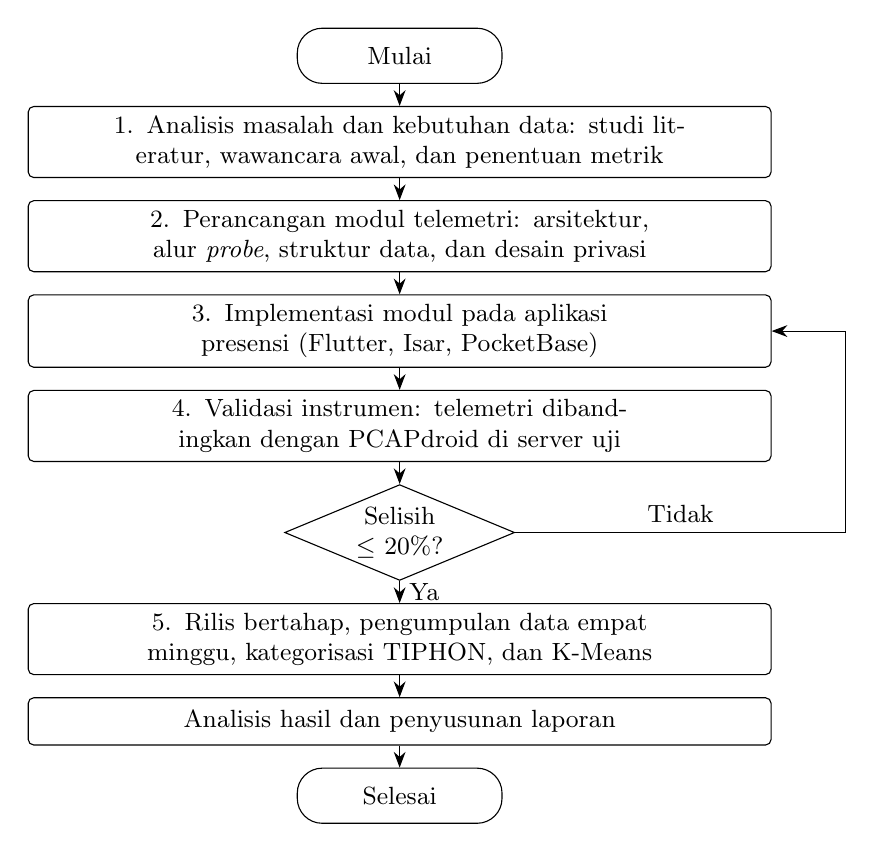
\begin{tikzpicture}[
    node distance=0.28cm,
    proses/.style={rectangle, draw, rounded corners=2pt, align=center, text width=9.2cm, minimum height=0.6cm, font=\small},
    batas/.style={rectangle, draw, rounded corners=9pt, align=center, minimum width=2.6cm, minimum height=0.7cm, font=\small},
    keputusan/.style={diamond, draw, aspect=2.4, align=center, inner sep=1pt, font=\small},
    panah/.style={-{Stealth[length=2mm]}}
]
\node[batas] (mulai) {Mulai};
\node[proses, below=of mulai] (s1) {1. Analisis masalah dan kebutuhan data: studi literatur, wawancara awal, dan penentuan metrik};
\node[proses, below=of s1] (s2) {2. Perancangan modul telemetri: arsitektur, alur \textit{probe}, struktur data, dan desain privasi};
\node[proses, below=of s2] (s3) {3. Implementasi modul pada aplikasi presensi (Flutter, Isar, PocketBase)};
\node[proses, below=of s3] (s4) {4. Validasi instrumen: telemetri dibandingkan dengan PCAPdroid di server uji};
\node[keputusan, below=of s4] (k) {Selisih\\$\le$ 20\%?};
\node[proses, below=of k] (s5) {5. Rilis bertahap, pengumpulan data empat minggu, kategorisasi TIPHON, dan K-Means};
\node[proses, below=of s5] (s6) {Analisis hasil dan penyusunan laporan};
\node[batas, below=of s6] (selesai) {Selesai};
\draw[panah] (mulai) -- (s1);
\draw[panah] (s1) -- (s2);
\draw[panah] (s2) -- (s3);
\draw[panah] (s3) -- (s4);
\draw[panah] (s4) -- (k);
\draw[panah] (k) -- node[right, font=\small] {Ya} (s5);
\draw[panah] (s5) -- (s6);
\draw[panah] (s6) -- (selesai);
\draw[panah] (k.east) -- node[above, font=\small] {Tidak} ++(4.2,0) |- (s3.east);
\end{tikzpicture}
\caption{Tahapan Penelitian}
\label{fig:tahapan}
\end{figure}

Berdasarkan Gambar~\ref{fig:tahapan} dapat dinyatakan bahwa penelitian terdiri atas lima tahap, dengan penjelasan sebagai berikut.
\begin{enumerate}
    \item \textbf{Analisis masalah dan kebutuhan data.} Peneliti mempelajari penelitian terdahulu, menggali keluhan presensi gagal terkirim dari HRD, dan menetapkan metrik yang diukur beserta rumusnya.
    \item \textbf{Perancangan modul telemetri.} Peneliti merancang arsitektur modul, alur \textit{probe}, struktur koleksi \texttt{net\_samples}, saklar jarak jauh, dan mekanisme anonimisasi.
    \item \textbf{Implementasi.} Modul dibuat sebagai komponen terpisah di dalam aplikasi presensi. Perubahan pada kode lama hanya berupa titik sadap kecil pada antrean sinkronisasi dan pemantau koneksi, dan seluruhnya diuji dengan pengujian unit.
    \item \textbf{Validasi instrumen.} Hasil telemetri dibandingkan dengan PCAPdroid pada kondisi jaringan yang dibuat sendiri di server uji. Jika selisih median RTT lebih dari 20\%, modul diperbaiki dan diuji kembali. Beban kuota dan baterai juga diukur pada tahap ini.
    \item \textbf{Rilis bertahap, pengumpulan data, dan analisis.} Aplikasi dirilis dengan telemetri dalam keadaan mati, lalu dinyalakan dari server untuk beberapa karyawan sebagai pilot selama dua hari sebelum dinyalakan untuk semua. Data dikumpulkan selama empat minggu, kemudian dibersihkan, dikategorikan dengan TIPHON, dan dikelompokkan dengan K-Means.
\end{enumerate}

\section{Desain Sistem}

\subsection{Analisis Kebutuhan Modul Telemetri}
Modul telemetri harus mengukur kualitas jaringan tanpa mengganggu fungsi utama aplikasi, yaitu presensi. Kebutuhan fungsional modul ditunjukkan pada Tabel~\ref{tab:kebutuhan}.

\begin{table}[!htb]
\centering
\caption{Kebutuhan Fungsional Modul Telemetri}
\label{tab:kebutuhan}
\begin{tabular}{>{\centering\arraybackslash}p{1.2cm}>{\raggedright\arraybackslash}p{12.09cm}}
\toprule
\textbf{Kode} & \textbf{Kebutuhan Fungsional} \\ \midrule
F01 & Menjalankan \textit{probe} tiga permintaan ke \texttt{/api/health} paling sering setiap 15 menit dan mencatat RTT serta \textit{jitter} \\ \garis
F02 & Mencatat hasil, lama, ukuran data, dan jenis galat setiap percobaan sinkronisasi presensi \\ \garis
F03 & Mencatat lama putus koneksi ketika perangkat kembali terhubung \\ \garis
F04 & Mencatat jenis jaringan, Wi-Fi kantor atau bukan, kode lokasi kerja, mode presensi, status lokasi terverifikasi, versi aplikasi, dan model perangkat pada setiap sampel \\ \garis
F05 & Menyimpan sampel di basis data lokal Isar dengan batas 2.000 sampel \\ \garis
F06 & Mengunggah sampel ke koleksi \texttt{net\_samples} secara berkelompok setelah antrean presensi kosong \\ \garis
F07 & Menyala atau mati berdasarkan saklar di aplikasi dan saklar di server (\texttt{app\_config}) \\ \garis
F08 & Mengganti identitas pengguna dengan kode anonim \\ \bottomrule
\end{tabular}
\par\vspace{3pt}
{\raggedright\footnotesize Sumber: diolah peneliti, 2026\par}
\end{table}

Kebutuhan nonfungsional modul adalah: (1) modul hanya mengamati dan tidak mengubah urutan, jeda, isi, maupun hasil sinkronisasi presensi; (2) setiap fungsi modul dibungkus penanganan galat sehingga kegagalan telemetri tidak menjalar ke alur presensi; (3) ukuran satu sampel kurang dari 300 \textit{byte} dan beban data telemetri kurang dari 1 MB per hari per perangkat; serta (4) modul dalam keadaan mati secara bawaan dan dapat dimatikan dari server tanpa memperbarui aplikasi.

\subsection{Arsitektur Modul Telemetri}
Hubungan antara alur presensi yang sudah ada, modul telemetri, dan server ditunjukkan pada Gambar~\ref{fig:arsitektur}.

\begin{figure}[!htb]
\centering
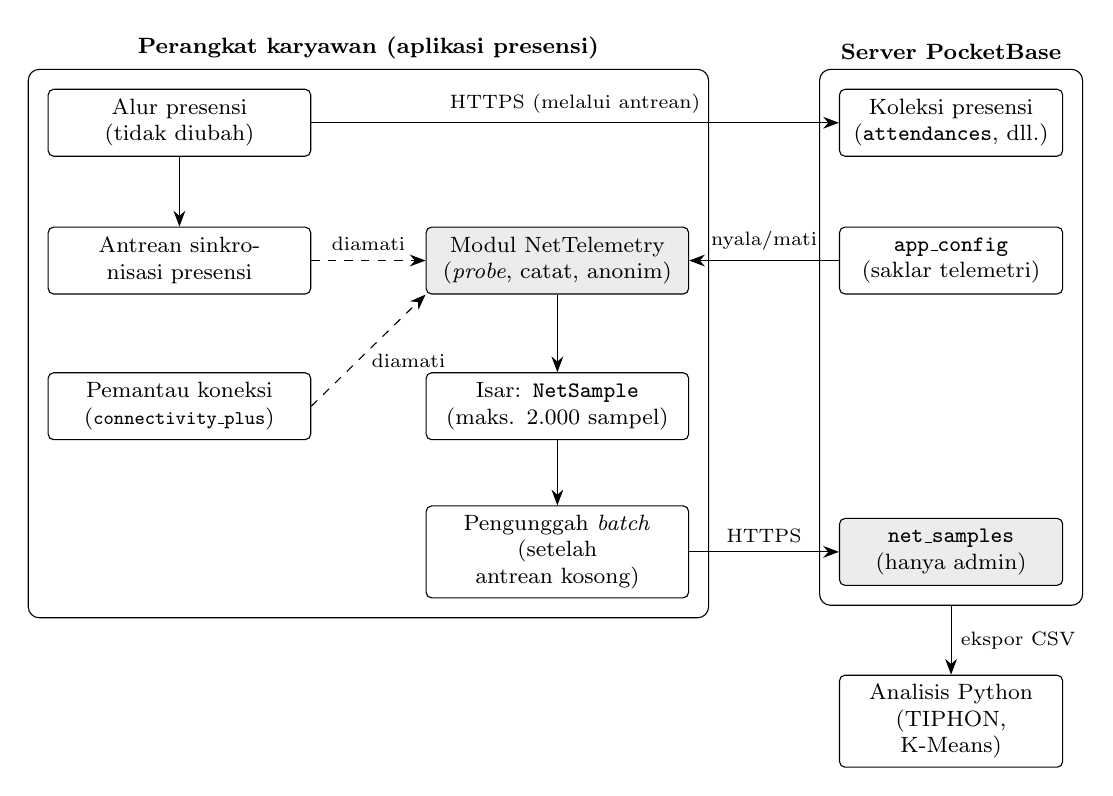
\begin{tikzpicture}[
    kotak/.style={rectangle, draw, rounded corners=2pt, align=center, text width=3.1cm, minimum height=0.85cm, font=\footnotesize},
    kotakserver/.style={rectangle, draw, rounded corners=2pt, align=center, text width=2.6cm, minimum height=0.85cm, font=\footnotesize},
    panah/.style={-{Stealth[length=2mm]}},
    amati/.style={-{Stealth[length=2mm]}, dashed}
]
% Perangkat karyawan
\node[kotak] (presensi) at (0,0) {Alur presensi\\(tidak diubah)};
\node[kotak] (antrean) at (0,-1.75) {Antrean sinkronisasi presensi};
\node[kotak] (koneksi) at (0,-3.6) {Pemantau koneksi\\({\scriptsize\texttt{connectivity\_plus}})};
\node[kotak, fill=gray!15] (telemetri) at (4.8,-1.75) {Modul NetTelemetry\\(\textit{probe}, catat, anonim)};
\node[kotak] (isar) at (4.8,-3.6) {Isar: \texttt{NetSample}\\(maks. 2.000 sampel)};
\node[kotak] (unggah) at (4.8,-5.45) {Pengunggah \textit{batch}\\(setelah antrean kosong)};
\begin{scope}[on background layer]
\node[draw, rounded corners=4pt, inner sep=7pt, fit=(presensi)(koneksi)(telemetri)(unggah), label={[font=\footnotesize\bfseries]above:Perangkat karyawan (aplikasi presensi)}] (hp) {};
\end{scope}
% Server
\node[kotakserver] (att) at (9.8,0) {Koleksi presensi\\(\texttt{attendances}, dll.)};
\node[kotakserver] (cfg) at (9.8,-1.75) {\texttt{app\_config}\\(saklar telemetri)};
\node[kotakserver, fill=gray!15] (net) at (9.8,-5.45) {\texttt{net\_samples}\\(hanya admin)};
\node[draw, rounded corners=4pt, inner sep=7pt, fit=(att)(cfg)(net), label={[font=\footnotesize\bfseries]above:Server PocketBase}] (srv) {};
\node[kotakserver] (py) at (9.8,-7.6) {Analisis Python\\(TIPHON, K-Means)};
% Panah
\draw[panah] (presensi) -- (antrean);
\draw[panah] (presensi) -- node[above, font=\scriptsize, pos=0.5] {HTTPS (melalui antrean)} (att);
\draw[amati] (antrean) -- node[above, font=\scriptsize] {diamati} (telemetri);
\draw[amati] (koneksi.east) -- node[below right, font=\scriptsize, inner sep=1pt] {diamati} (telemetri.south west);
\draw[panah] (telemetri) -- (isar);
\draw[panah] (isar) -- (unggah);
\draw[panah] (unggah) -- node[above, font=\scriptsize] {HTTPS} (net);
\draw[panah] (cfg) -- node[above, font=\scriptsize] {nyala/mati} (telemetri);
\draw[panah] (srv.south -| net) -- node[right, font=\scriptsize] {ekspor CSV} (py);
\end{tikzpicture}
\caption{Arsitektur Modul Telemetri pada Aplikasi Presensi}
\label{fig:arsitektur}
\end{figure}

Berdasarkan Gambar~\ref{fig:arsitektur} dapat dinyatakan bahwa modul telemetri berdiri di samping alur presensi, bukan di dalamnya. Garis putus-putus menunjukkan bahwa modul hanya mengamati antrean sinkronisasi dan pemantau koneksi. Sampel disimpan di Isar lalu diunggah ke koleksi \texttt{net\_samples} dengan prioritas terendah, yaitu setelah seluruh data presensi terkirim. Modul hanya aktif jika saklar di aplikasi dan saklar \texttt{app\_config} di server sama-sama menyala, sehingga jika terjadi masalah, seluruh perangkat dapat dihentikan dari server tanpa merilis aplikasi baru.

\subsection{Alur Pengukuran Probe}
Alur pengukuran \textit{probe} yang dijalankan pada setiap akhir siklus sinkronisasi ditunjukkan pada Gambar~\ref{fig:alur_probe}.

\begin{figure}[!htb]
\centering
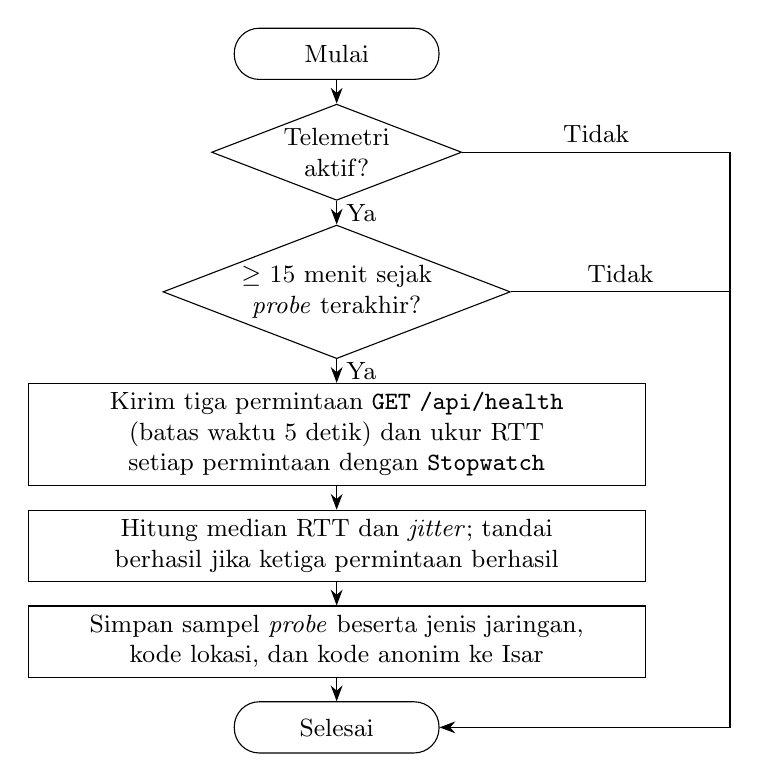
\begin{tikzpicture}[
    node distance=0.3cm,
    proses/.style={rectangle, draw, align=center, text width=7.6cm, minimum height=0.55cm, font=\small},
    batas/.style={rectangle, draw, rounded corners=9pt, align=center, minimum width=2.6cm, minimum height=0.65cm, font=\small},
    keputusan/.style={diamond, draw, aspect=2.6, align=center, inner sep=1pt, font=\small},
    panah/.style={-{Stealth[length=2mm]}}
]
\node[batas] (a) {Mulai};
\node[keputusan, below=of a] (k1) {Telemetri\\aktif?};
\node[keputusan, below=of k1] (k2) {$\ge$ 15 menit sejak\\\textit{probe} terakhir?};
\node[proses, below=of k2] (b) {Kirim tiga permintaan \texttt{GET /api/health} (batas waktu 5 detik) dan ukur RTT setiap permintaan dengan \texttt{Stopwatch}};
\node[proses, below=of b] (c) {Hitung median RTT dan \textit{jitter}; tandai berhasil jika ketiga permintaan berhasil};
\node[proses, below=of c] (d) {Simpan sampel \textit{probe} beserta jenis jaringan, kode lokasi, dan kode anonim ke Isar};
\node[batas, below=of d] (e) {Selesai};
\foreach \x/\y in {a/k1,b/c,c/d,d/e} \draw[panah] (\x) -- (\y);
\draw[panah] (k1) -- node[right, font=\small] {Ya} (k2);
\draw[panah] (k2) -- node[right, font=\small] {Ya} (b);
\draw[panah] (k1.east) -- node[above, font=\small] {Tidak} ++(3.4,0) coordinate (jalur) |- (e.east);
\draw (k2.east) -- node[above, font=\small] {Tidak} (k2.east -| jalur);
\end{tikzpicture}
\caption{Alur Pengukuran \textit{Probe} pada Modul Telemetri}
\label{fig:alur_probe}
\end{figure}

Berdasarkan Gambar~\ref{fig:alur_probe} dapat dinyatakan bahwa \textit{probe} tidak dijalankan pada setiap siklus sinkronisasi, tetapi paling sering satu kali setiap 15 menit. Batasan ini menjaga beban kuota dan baterai tetap kecil. Satu sampel \textit{probe} menghasilkan satu nilai \textit{delay}, satu nilai \textit{jitter}, dan satu status berhasil atau gagal.

\subsection{Rancangan Data}
Setiap sampel disimpan di koleksi \texttt{net\_samples} pada server PocketBase dengan struktur yang ditunjukkan pada Tabel~\ref{tab:net_samples}.

\begin{table}[!htb]
\centering
\caption{Struktur Koleksi \texttt{net\_samples}}
\label{tab:net_samples}
\begin{tabular}{>{\raggedright\arraybackslash}p{3.1cm}>{\centering\arraybackslash}p{1.9cm}>{\raggedright\arraybackslash}p{7.94cm}}
\toprule
\textbf{Kolom} & \textbf{Tipe} & \textbf{Keterangan} \\ \midrule
\texttt{anon\_id} & teks & 16 karakter pertama SHA-256 dari ID pengguna dan \textit{salt} rahasia \\ \garis
\texttt{kind} & pilihan & \texttt{probe}, \texttt{sync\_attempt}, atau \texttt{outage} \\ \garis
\texttt{office\_id} & teks & Kode lokasi kerja dari presensi terakhir \\ \garis
\texttt{mode} & pilihan & Mode presensi: \texttt{normal}, \texttt{titik\_admin}, \texttt{gamas}, atau \texttt{fleksibel} \\ \garis
\texttt{loc\_valid} & \textit{boolean} & Benar jika sampel diambil paling lama 15 menit sebelum atau sesudah presensi yang lolos \textit{geofence} \\ \garis
\texttt{network\_type} & pilihan & \texttt{wifi}, \texttt{mobile}, \texttt{ethernet}, \texttt{none}, atau \texttt{other} \\ \garis
\texttt{office\_wifi} & \textit{boolean} & Benar jika Wi-Fi yang terhubung adalah Wi-Fi kantor (BSSID tidak disimpan) \\ \garis
\texttt{rtt\_ms}, \texttt{jitter\_ms} & angka & RTT dan \textit{jitter} \textit{probe}, atau lama permintaan sinkronisasi \\ \garis
\texttt{ok}, \texttt{error\_class} & \textit{boolean}, pilihan & Status berhasil dan jenis galat (\texttt{timeout}, \texttt{network}, \texttt{http4xx}, \texttt{http5xx}) \\ \garis
\texttt{bytes\_sent} & angka & Ukuran data terkirim pada percobaan sinkronisasi \\ \garis
\texttt{outage\_ms} & angka & Lama putus koneksi \\ \garis
\texttt{sampled\_at} & tanggal & Waktu pengukuran (UTC) \\ \garis
\texttt{app\_version}, \texttt{os\_sdk}, \texttt{device\_model} & teks, angka & Versi aplikasi, versi Android, dan model perangkat (bukan nomor seri) \\ \bottomrule
\end{tabular}
\par\vspace{3pt}
{\raggedright\footnotesize Sumber: diolah peneliti, 2026\par}
\end{table}

Berdasarkan Tabel~\ref{tab:net_samples} dapat dinyatakan bahwa tidak ada kolom yang menyimpan nama, email, ID pengguna asli, koordinat GPS, maupun foto. Aturan akses koleksi dibuat sehingga karyawan hanya dapat menambah data, sedangkan melihat, mengubah, dan menghapus data hanya dapat dilakukan oleh admin. Kode anonim tetap memungkinkan analisis membedakan perangkat tanpa mengetahui pemiliknya, sesuai prinsip pemrosesan data yang terbatas dan spesifik \parencite{uupdp2022}.

\section{Alat Penelitian}
Alat yang digunakan dalam penelitian ini terdiri dari perangkat keras dan perangkat lunak yang ditunjukkan pada Tabel~\ref{tab:alat}.

\begin{table}[!htb]
\centering
\caption{Alat Penelitian}
\label{tab:alat}
\begin{tabular}{>{\raggedright\arraybackslash}p{4.2cm}>{\raggedright\arraybackslash}p{9.09cm}}
\toprule
\textbf{Alat} & \textbf{Kegunaan} \\ \midrule
\multicolumn{2}{l}{\textbf{Perangkat keras}} \\ \garis
Laptop (Windows 11) & Pengembangan modul, pengolahan data, dan penulisan laporan \\ \garis
Minimal dua ponsel Android berbeda kelas & Pengujian modul dan validasi instrumen \\ \garis
Server PocketBase produksi dan server uji & Penyimpanan data presensi dan sampel telemetri \\ \garis
\multicolumn{2}{l}{\textbf{Perangkat lunak}} \\ \garis
Flutter dan Dart & \textit{Framework} dan bahasa pemrograman aplikasi presensi \\ \garis
Isar 3.1 & Basis data lokal untuk menyimpan sampel sebelum diunggah \\ \garis
\texttt{connectivity\_plus} & Mendeteksi jenis jaringan dan perubahan status koneksi \\ \garis
PCAPdroid dan Wireshark & Merekam dan membaca lalu lintas jaringan untuk validasi instrumen \\ \garis
Android Debug Bridge (adb) & Mengatur skenario Wi-Fi, data seluler, dan mode pesawat saat validasi \\ \garis
Python (pandas, scikit-learn, matplotlib) & Pembersihan data, kategorisasi TIPHON, K-Means, dan pembuatan grafik \\ \garis
Visual Studio Code & Penyunting kode \\ \bottomrule
\end{tabular}
\par\vspace{3pt}
{\raggedright\footnotesize Sumber: diolah peneliti, 2026\par}
\end{table}

\section{Teknik Analisis Data}
Analisis data dilakukan dalam lima langkah, yaitu validasi instrumen, pembersihan dan agregasi data, kategorisasi TIPHON, pengelompokan dengan K-Means, dan perbandingan hasil. Karena data penelitian baru diperoleh setelah modul dirilis, contoh perhitungan pada subbab ini menggunakan data ilustrasi.

\subsection{Validasi Instrumen}
Validasi dilakukan dengan membandingkan median RTT telemetri dan median RTT tingkat TCP dari PCAPdroid pada setiap kondisi jaringan:
\begin{equation}
\delta = \frac{\left| \tilde{d}_{\mathrm{telemetri}} - \tilde{d}_{\mathrm{PCAP}} \right|}{\tilde{d}_{\mathrm{PCAP}}} \times 100\%
\label{eq:validasi}
\end{equation}
dengan $\delta$ adalah selisih relatif, $\tilde{d}_{\mathrm{telemetri}}$ adalah median RTT dari telemetri, dan $\tilde{d}_{\mathrm{PCAP}}$ adalah median RTT dari PCAPdroid. Telemetri mengukur di tingkat aplikasi sehingga termasuk waktu pemrosesan HTTP, sedangkan PCAPdroid mengukur di tingkat TCP, sehingga selisih kecil pasti ada. Instrumen dinyatakan valid jika $\delta \le 20\%$ pada setiap kondisi. Sebagai pembanding, MopEye yang mengukur di tingkat paket memiliki selisih rata-rata RTT paling banyak 1 ms terhadap tcpdump \parencite{wu2017mopeye}. Selain itu, lama putus koneksi yang tercatat harus sesuai dengan jadwal skenario dengan toleransi lima detik, dan beban data telemetri harus kurang dari 1 MB per hari per perangkat.

\subsection{Pembersihan dan Agregasi Data}
Sampel dibersihkan dengan membuang sampel yang nilai RTT-nya kurang dari atau sama dengan 0 atau lebih dari 60.000 ms dan sampel ganda. Sampel dengan jenis jaringan \texttt{none} tidak dibuang, karena lokasi tanpa sinyal sama sekali adalah kondisi terburuk; sampel tersebut dihitung sebagai persentase waktu tanpa jaringan per lokasi. Sampel yang bersih kemudian dikelompokkan per kombinasi lokasi kerja, jenis jaringan, dan slot waktu, yaitu pagi (05.00--09.00), siang (09.00--15.00), sore (15.00--19.00), dan malam (19.00--05.00). Setiap kombinasi disebut agregat. Nilai setiap agregat adalah median \textit{delay}, median \textit{jitter}, tingkat kegagalan, dan median \textit{throughput}. Median dipilih agar hasil tidak mudah dipengaruhi gangguan sesaat, sejalan dengan saran \textcite{tripkovic2021cluster} untuk mengelompokkan dan merata-ratakan pengukuran \textit{crowdsourcing} sebelum dianalisis. Agregat dengan kurang dari sepuluh sampel \textit{probe} tidak diikutkan dalam K-Means, tetapi tetap dilaporkan secara deskriptif.

Kode lokasi pada sampel hanya dapat dipercaya jika perangkat memang berada di lokasi itu saat sampel diambil. Karena itu, analisis per lokasi hanya memakai sampel dengan \texttt{loc\_valid} bernilai benar, yaitu sampel yang diambil paling lama 15 menit dari presensi yang lolos \textit{geofence}. Presensi \textit{offline} yang baru terkirim beberapa jam kemudian dinilai menurut waktu pengirimannya, sehingga tidak dianggap berasal dari lokasi presensi. Sampel mode GAMAS dan lokasi fleksibel dianalisis terpisah sebagai kelompok ``di luar lokasi kerja'', sedangkan sampel tanpa lokasi terverifikasi tetap dipakai untuk analisis per jenis jaringan dan waktu. Karena karyawan bebas memilih Wi-Fi atau data seluler, jumlah sampel setiap jenis jaringan per lokasi dilaporkan, dan Wi-Fi kantor dibedakan dari Wi-Fi lain.

\subsection{Kategorisasi TIPHON}
Setiap metrik agregat dikonversi ke indeks 1--4 menurut Tabel~\ref{tab:tiphon}, lalu indeks keseluruhan dihitung sebagai rata-rata keempat indeks dan ditafsirkan dengan Tabel~\ref{tab:tiphon_total}. Contoh dengan enam agregat ilustrasi ditunjukkan pada Tabel~\ref{tab:ilustrasi_tiphon}.

\begin{table}[!htb]
\centering
\caption{Contoh Kategorisasi TIPHON pada Data Ilustrasi}
\label{tab:ilustrasi_tiphon}
\begin{tabular}{>{\centering\arraybackslash}p{0.9cm}>{\raggedright\arraybackslash}p{3.4cm}>{\centering\arraybackslash}p{1.25cm}>{\centering\arraybackslash}p{1.25cm}>{\centering\arraybackslash}p{1.25cm}>{\centering\arraybackslash}p{1.85cm}>{\centering\arraybackslash}p{1.6cm}}
\toprule
\textbf{Kode} & \textbf{Agregat} & \textbf{\textit{Delay} (ms)} & \textbf{\textit{Jitter} (ms)} & \textbf{Gagal (\%)} & \textbf{\textit{Throughput} (kbps)} & \textbf{Rata-rata Indeks} \\ \midrule
G1 & Kantor, Wi-Fi, pagi & 85 (4) & 12 (3) & 0,5 (4) & 3.200 (4) & 3,75 \\ \garis
G2 & Kantor, seluler, pagi & 140 (4) & 35 (3) & 2,0 (4) & 1.900 (3) & 3,50 \\ \garis
G3 & Posko A, seluler, pagi & 320 (2) & 95 (2) & 9,0 (3) & 850 (2) & 2,25 \\ \garis
G4 & Posko A, seluler, sore & 510 (1) & 160 (1) & 21,0 (2) & 420 (1) & 1,25 \\ \garis
G5 & Gudang, Wi-Fi, siang & 180 (3) & 40 (3) & 3,5 (3) & 1.500 (3) & 3,00 \\ \garis
G6 & Posko B, seluler, sore & 460 (1) & 140 (1) & 17,0 (2) & 600 (1) & 1,25 \\ \bottomrule
\end{tabular}
\par\vspace{3pt}
{\raggedright\footnotesize Catatan: angka dalam kurung adalah indeks TIPHON.\\ Sumber: data ilustrasi, diolah peneliti, 2026\par}
\end{table}

Berdasarkan Tabel~\ref{tab:ilustrasi_tiphon} dapat dinyatakan bahwa G1, G2, dan G5 termasuk kategori memuaskan, G3 kurang memuaskan, sedangkan G4 dan G6 tidak memuaskan. Kategorisasi ini menilai setiap metrik secara terpisah, sehingga satu agregat dapat bernilai baik pada satu metrik tetapi buruk pada metrik lain, seperti G3 yang tingkat kegagalannya bagus tetapi \textit{delay}-nya sedang.

\subsection{Pengelompokan dengan K-Means}
Pengelompokan dilakukan dengan langkah-langkah pada Subbab~\ref{subsec:kmeans}. Atribut yang digunakan adalah keempat metrik agregat. Setiap atribut dinormalisasi dengan RobustScaler menggunakan Persamaan~(\ref{eq:robust}), K-Means dijalankan dengan inisialisasi k-means++ sebanyak sepuluh kali untuk setiap nilai $k$, dan hasil dengan SSE terkecil dipilih. Nilai $k$ yang diuji adalah 2 sampai 6, lalu $k$ terbaik ditentukan dengan metode \textit{elbow} dan nilai \textit{silhouette} tertinggi seperti dijelaskan pada Subbab~\ref{subsec:jumlah_klaster}. Dugaan awal adalah $k = 3$, yaitu kualitas baik, sedang, dan buruk, tetapi nilai akhirnya ditentukan oleh data.

Agar perhitungan mudah diikuti, contoh berikut hanya menggunakan dua atribut, yaitu \textit{delay} dan tingkat kegagalan dari Tabel~\ref{tab:ilustrasi_tiphon}, dengan $k = 2$. Untuk atribut \textit{delay}, nilai $Q_1 = 150$, $Q_2 = 250$, dan $Q_3 = 425$, sehingga normalisasi G1 adalah:
\begin{equation*}
x'_{\mathrm{G1,delay}} = \frac{85 - 250}{425 - 150} = -0{,}6000
\end{equation*}
Untuk atribut tingkat kegagalan, nilai $Q_1 = 2{,}375$, $Q_2 = 6{,}25$, dan $Q_3 = 15$, sehingga $x'_{\mathrm{G1,gagal}} = (0{,}5 - 6{,}25)/12{,}625 = -0{,}4554$. Hasil normalisasi seluruh agregat ditunjukkan pada Tabel~\ref{tab:ilustrasi_kmeans}. Pusat awal dipilih G1 dan G4. Jarak G3 ke pusat pertama dihitung dengan Persamaan~(\ref{eq:euclidean}):
\begin{equation*}
D(\mathrm{G3}, c_1) = \sqrt{(0{,}2545 - (-0{,}6000))^2 + (0{,}2178 - (-0{,}4554))^2} = 1{,}0879
\end{equation*}

\begin{table}[!htb]
\centering
\caption{Contoh Normalisasi dan Iterasi Pertama K-Means}
\label{tab:ilustrasi_kmeans}
\begin{tabular}{>{\centering\arraybackslash}p{0.9cm}>{\centering\arraybackslash}p{1.55cm}>{\centering\arraybackslash}p{1.55cm}>{\centering\arraybackslash}p{1.55cm}>{\centering\arraybackslash}p{1.55cm}>{\centering\arraybackslash}p{1.3cm}>{\centering\arraybackslash}p{3.13cm}}
\toprule
\textbf{Kode} & \textbf{$x'_{\mathrm{delay}}$} & \textbf{$x'_{\mathrm{gagal}}$} & \textbf{$D(x, c_1)$} & \textbf{$D(x, c_2)$} & \textbf{Klaster} & \textbf{Kategori TIPHON} \\ \midrule
G1 & $-$0,6000 & $-$0,4554 & 0,0000 & 2,2417 & 1 & Memuaskan \\ \garis
G2 & $-$0,4000 & $-$0,3366 & 0,2326 & 2,0187 & 1 & Memuaskan \\ \garis
G3 & 0,2545 & 0,2178 & 1,0879 & 1,1751 & 1 & Kurang memuaskan \\ \garis
G4 & 0,9455 & 1,1683 & 2,2417 & 0,0000 & 2 & Tidak memuaskan \\ \garis
G5 & $-$0,2545 & $-$0,2178 & 0,4193 & 1,8334 & 1 & Memuaskan \\ \garis
G6 & 0,7636 & 0,8515 & 1,8888 & 0,3653 & 2 & Tidak memuaskan \\ \bottomrule
\end{tabular}
\par\vspace{3pt}
{\raggedright\footnotesize Sumber: data ilustrasi, diolah peneliti, 2026\par}
\end{table}

Pusat klaster baru dihitung dengan Persamaan~(\ref{eq:centroid}), yaitu $c_1 = (-0{,}2500;\ -0{,}1980)$ dari G1, G2, G3, dan G5, serta $c_2 = (0{,}8545;\ 1{,}0099)$ dari G4 dan G6. Pada iterasi kedua, anggota setiap klaster tidak berubah sehingga iterasi berhenti. Berdasarkan Tabel~\ref{tab:ilustrasi_kmeans} dapat dinyatakan bahwa klaster 2 berisi agregat posko dengan jaringan seluler pada sore hari yang \textit{delay} dan tingkat kegagalannya tinggi. G3 masuk klaster 1 walaupun kategori TIPHON-nya kurang memuaskan, dan jaraknya ke kedua pusat hampir sama (1,0879 dan 1,1751). Hal ini menunjukkan bahwa dengan $k = 2$ agregat yang berkualitas sedang belum terpisah, sehingga nilai $k$ perlu diuji lebih dari satu. Pada data penelitian, perhitungan ini dilakukan dengan scikit-learn menggunakan keempat atribut, lalu setiap klaster diberi label berdasarkan nilai pusatnya.

\subsection{Perbandingan Hasil Klaster}
Hasil K-Means dibandingkan dengan kategori TIPHON menggunakan tabel silang antara label klaster dan kategori indeks keseluruhan. Kategori memuaskan dan sangat memuaskan dipadankan dengan klaster berkualitas baik, kategori kurang memuaskan dengan klaster sedang, dan kategori tidak memuaskan dengan klaster buruk. Tingkat kesesuaian dihitung dengan persamaan berikut:
\begin{equation}
K = \frac{\text{jumlah agregat yang label klasternya sesuai kategori TIPHON}}{\text{jumlah seluruh agregat}} \times 100\%
\label{eq:kesesuaian}
\end{equation}
Selain itu, lokasi kerja yang masuk klaster buruk dicocokkan dengan keterangan HRD tentang lokasi yang sering sulit sinyal. Ketidaksesuaian tidak dianggap kegagalan, tetapi dibahas penyebabnya, misalnya ambang TIPHON yang terlalu ketat atau persepsi HRD yang berbeda dengan data. Hasil disajikan dalam tabel statistik per lokasi, diagram kotak \textit{delay}, grafik sebaran klaster, dan peta panas jam terhadap lokasi.

\section{Jadwal Penelitian}
\label{sec:jadwal}
Penelitian direncanakan selama tiga bulan atau 12 minggu, seperti ditunjukkan pada Tabel~\ref{tab:jadwal}.

\begin{table}[!htb]
\centering
\caption{Jadwal Penelitian}
\label{tab:jadwal}
\newcommand{\isi}{\cellcolor{gray!60}}
\setlength{\tabcolsep}{1.5pt}
\begin{tabular}{>{\centering\arraybackslash}p{0.6cm}>{\raggedright\arraybackslash}p{3.9cm}*{12}{>{\centering\arraybackslash}p{0.38cm}}}
\toprule
\textbf{No.} & \textbf{Kegiatan} & \multicolumn{4}{c}{\textbf{Bulan ke-1}} & \multicolumn{4}{c}{\textbf{Bulan ke-2}} & \multicolumn{4}{c}{\textbf{Bulan ke-3}} \\ \cmidrule(lr){3-6} \cmidrule(lr){7-10} \cmidrule(lr){11-14}
 & & \multicolumn{12}{c}{\textbf{Minggu ke-}} \\
 & & 1 & 2 & 3 & 4 & 5 & 6 & 7 & 8 & 9 & 10 & 11 & 12 \\ \midrule
1. & Studi literatur dan proposal & \isi &  &  &  &  &  &  &  &  &  &  &  \\ \garis
2. & Ujian proposal dan izin penelitian &  & \isi &  &  &  &  &  &  &  &  &  &  \\ \garis
3. & Perancangan modul telemetri &  & \isi & \isi &  &  &  &  &  &  &  &  &  \\ \garis
4. & Implementasi dan pengujian modul &  &  & \isi & \isi & \isi &  &  &  &  &  &  &  \\ \garis
5. & Validasi instrumen di server uji &  &  &  &  & \isi & \isi &  &  &  &  &  &  \\ \garis
6. & Rilis bertahap dan pilot &  &  &  &  &  & \isi &  &  &  &  &  &  \\ \garis
7. & Pengumpulan data dan wawancara HRD &  &  &  &  &  &  & \isi & \isi & \isi & \isi &  &  \\ \garis
8. & Analisis data (TIPHON dan K-Means) &  &  &  &  &  &  &  &  &  & \isi & \isi &  \\ \garis
9. & Penyusunan laporan skripsi &  &  &  &  &  &  &  &  &  & \isi & \isi & \isi \\ \bottomrule
\end{tabular}
\par\vspace{3pt}
{\raggedright\footnotesize Sumber: diolah peneliti, 2026\par}
\end{table}

    %===========================================================

    %===========================================================
    % Daftar Pustaka (APA)
    %-----------------------------------------------------------
    \tocchapter{DAFTAR PUSTAKA}
    \printbibliography[title={DAFTAR PUSTAKA}]
    %===========================================================

    % Lampiran (Pedoman 4.1 no. 3: bagian akhir proposal)
    \pagebreak
    \chapter*{LAMPIRAN}
\phantomsection
\addcontentsline{toc}{chapter}{LAMPIRAN}

% Lampiran tidak diberi nomor tabel agar Daftar Tabel hanya memuat tabel Bab 1-3.
\newcommand{\judullampiran}[1]{\par\medskip\phantomsection\addcontentsline{toc}{section}{#1}\noindent\textbf{#1}\par\smallskip}

\judullampiran{Lampiran 1. Pedoman Wawancara HRD}
Wawancara dilakukan dengan satu orang HRD atau admin presensi, secara langsung atau melalui pesan, setelah izin penelitian dari perusahaan diperoleh. Jawaban dicatat apa adanya dan tidak menyebut nama karyawan.

{\small\singlespacing
\setlength{\tabcolsep}{5pt}
\begin{longtable}{>{\centering\arraybackslash}p{0.8cm}>{\raggedright\arraybackslash}p{12.49cm}}
\toprule
\textbf{No.} & \textbf{Pertanyaan} \\ \midrule
1. & Lokasi kerja (kantor, posko, atau gudang) mana saja yang paling sering dikeluhkan karyawan karena presensi lambat atau gagal terkirim? \\ \garis
2. & Pada jam berapa keluhan tersebut paling sering muncul? \\ \garis
3. & Di lokasi tersebut, karyawan biasanya memakai Wi-Fi kantor atau data seluler? Jika seluler, operator apa yang umum dipakai? \\ \garis
4. & Apakah ada lokasi yang menurut HRD sinyalnya baik tetapi tetap ada keluhan presensi? \\ \garis
5. & Bagaimana HRD menangani presensi yang terlambat masuk ke rekap karena masalah jaringan? \\ \garis
6. & Apakah perusahaan pernah atau berencana memasang Wi-Fi atau \textit{repeater} di lokasi tertentu? Jika ya, di mana? \\ \bottomrule
\end{longtable}
}

\judullampiran{Lampiran 2. Lembar Validasi Instrumen}
Lembar ini diisi untuk setiap kondisi jaringan pada server uji. Setiap baris adalah satu pasang pengukuran, yaitu RTT \textit{probe} dari telemetri dan RTT TCP pada waktu yang sama dari PCAPdroid.

\noindent Kondisi jaringan: Wi-Fi / seluler 4G / mode pesawat / putus-sambung \quad Perangkat: \dotfill \quad Tanggal: \dotfill

{\small\singlespacing
\setlength{\tabcolsep}{5pt}
\renewcommand{\arraystretch}{1.3}
\begin{longtable}{>{\centering\arraybackslash}p{0.9cm}>{\centering\arraybackslash}p{2.3cm}>{\centering\arraybackslash}p{3.0cm}>{\centering\arraybackslash}p{3.0cm}>{\raggedright\arraybackslash}p{3.04cm}}
\toprule
\textbf{No.} & \textbf{Jam} & \textbf{RTT Telemetri (ms)} & \textbf{RTT PCAPdroid (ms)} & \textbf{Catatan} \\ \midrule
1 & & & & \\ \garis
2 & & & & \\ \garis
3 & & & & \\ \garis
4 & & & & \\ \garis
5 & & & & \\ \garis
6 & & & & \\ \garis
7 & & & & \\ \garis
8 & & & & \\ \garis
9 & & & & \\ \garis
10 & & & & \\ \midrule
\multicolumn{2}{l}{Median} & & & \\ \garis
\multicolumn{2}{l}{Selisih relatif $\delta$} & \multicolumn{3}{l}{\dotfill\ \% (valid jika $\le$ 20\%)} \\ \bottomrule
\end{longtable}
}

\noindent Skenario putus-sambung: jadwal putus (detik) \dotfill\ \quad lama putus tercatat (detik) \dotfill\ \quad sesuai ($\pm$ 5 detik): ya / tidak

\noindent Beban telemetri selama 24 jam: data \dotfill\ KB \quad baterai (nyala/mati) \dotfill

\judullampiran{Lampiran 3. Teks Pemberitahuan pada Aplikasi}
Teks berikut ditampilkan pada menu Profil, bagian Tentang Aplikasi, selama periode pengumpulan data.

\begin{quote}\singlespacing\small
Aplikasi ini mencatat kualitas koneksi ke server, yaitu waktu respons, keberhasilan pengiriman, kecepatan unggah, dan lama koneksi terputus, untuk penelitian tentang kualitas jaringan di lokasi kerja. Data yang dicatat tidak memuat nama, email, lokasi GPS, maupun foto, dan identitas pengguna diganti dengan kode acak. Pencatatan ini tidak mengubah cara presensi dan dapat dihentikan oleh perusahaan kapan saja. Pengumpulan data telah disetujui oleh PT Semeru Agung Mandiri.
\end{quote}


\end{document}
